\documentclass[11pt,a4paper]{article}
\usepackage[margin=2.2cm]{geometry}
\usepackage[T1]{fontenc}
\usepackage{lmodern}
\usepackage{amsmath,amssymb}
\usepackage{booktabs}
\usepackage{graphicx}
\usepackage{caption}
\usepackage{subcaption}
\usepackage{enumitem}
\usepackage[colorlinks=true,allcolors=blue!50!black]{hyperref}
% Shared TikZ styles for the folded-surface-code layout pictures that gen_layout.py writes
% into figures/. Written by hand.
\usepackage{tikz}
\usetikzlibrary{arrows.meta,calc}
\definecolor{SwapCol}{HTML}{8E44AD}   % the purple of the LRB paper palette
\definecolor{TopNavy}{RGB}{16,16,120}
\tikzset{
  botline/.style={draw=black!45},
  topline/.style={draw=TopNavy},
  pairline/.style={draw=SwapCol},
  botanc/.style={draw=black!62,fill=black!7},
  topanc/.style={draw=TopNavy,fill=blue!10},
  foldq/.style={draw=black,fill=yellow!55},
  botq/.style={draw=black,fill=white},
  topq/.style={draw=black,fill=black!14},
  qlabel/.style={inner sep=0pt,text=black},
  anclabel/.style={inner sep=0pt},
  botanctext/.style={text=black!62},
  topanctext/.style={text=TopNavy},
  foldline/.style={draw=red!75!black,line width=0.9pt,dash pattern=on 4pt off 3pt},
  foldtext/.style={text=red!75!black,font=\footnotesize},
  dim/.style={draw=black!75,line width=0.4pt,{Latex[length=1.4mm,width=1.1mm]}-{Latex[length=1.4mm,width=1.1mm]}},
  dimtext/.style={font=\footnotesize,text=black!85,inner sep=2pt},
  panel/.style={font=\small},
}

\captionsetup{font=small,labelfont=bf}
\setlist{itemsep=2pt,topsep=4pt}
\makeatletter\newcommand{\rawinput}[1]{\@@input #1 }\makeatother

\title{\vspace{-1.2cm}A nearest-neighbour two-layer layout of the folded surface code\\ for every distance $d\ge 2$}
\author{}
\date{Working note, 24 November 2026}

\begin{document}
\maketitle
\vspace{-1.4cm}

\section{Summary}

This note places the qubits of the folded surface code in two interleaved layers so that every
coupler is short, for every distance $d\ge2$. A coupler joins two nearest neighbours of one
layer, a distance $a$ apart, or a site of one layer to a site of the other $a/\sqrt2$ away.
The code is the unrotated surface code
$[[d^2+(d-1)^2,\,1,\,d]]$, for qubits or qudits, folded along its diagonal. The fold brings
$(d-1)^2$ pairs of data qubits together, and the logical Hadamard and phase gates act on each
pair with a two-qubit gate~\cite{Moussa2016}. In the unfolded patch the two partners of a pair
sit up to $2\sqrt2\,(d-1)\,a$ apart, where $a$ is the pitch of the lattice. In the layout below
they sit $a/\sqrt2$ apart. The cost is $2(d-1)(2d-3)$ places
where two couplers cross.

The distance-3 member is the triangle of Fig.~\ref{fig:d3}(b), with 13 data qubits and 12
ancillas. The distance-2 member is
the five-qudit code of the LRB paper, with the same labels. Table~\ref{tab:counts} lists what a
chip of distance $d$ contains, and Sec.~\ref{sec:chip} lists what the fabrication has to provide.
Section~\ref{sec:memory} compares its memory under circuit-level noise with the rotated surface
code: the thresholds agree, the folded code needs 10 to 30\% more qubits for the same memory, and
in exchange its logical $H$ is free and its logical $S$ costs one layer of CZ gates.

\section{The code and the fold}

Put the patch on a square grid with sites $(x,y)$, $0\le x,y\le 2d-2$, with $x$ to the right
and $y$ downwards. Data qubits sit on the sites with $x+y$ even and check ancillas on the sites
with $x+y$ odd. An ancilla measures a product of Paulis on its nearest neighbours, of $X$ type
if $x$ is odd and of $Z$ type if $x$ is even. Ancillas on the edge of the patch have three
neighbours and all others have four. Logical $X$ acts on a column of even $x$ and logical $Z$ on
a row of even $y$. Each holds $d$ qubits. Figure~\ref{fig:d3}(a) shows the patch for $d=3$.

The fold is the reflection $(x,y)\leftrightarrow(y,x)$. It fixes the $2d-1$ data qubits on the
diagonal, called fold qubits here, and exchanges the other $2(d-1)^2$ in pairs. It sends every
$X$ check to a $Z$ check on the mirrored qubits. Because of this symmetry the Clifford gates are
transversal in the folded sense~\cite{Moussa2016,Breuckmann2024}. Logical $H$ is a Hadamard on
every data qubit and a SWAP on every pair. Logical $S$ is a phase gate on every fold qubit,
$S$ and $S^{-1}$ alternating along the fold, and a CZ on every pair. For qutrits the same gates
carry signs: $H$ on the sites with even coordinates and $H^{-1}$ on the sites with odd
coordinates, $S^{(-1)^k}$ on the fold qubit $(k,k)$, and $\mathrm{CZ}^{(-1)^x}$ on the pair of
$(x,y)$ with $x<y$. At $d=2$ these are the logical gates of the LRB paper,
$\bar H=(H_0H_1^{-1}H_2H_3H_4)\,\mathrm{SWAP}_{2,3}$ and
$\bar S=S_0S_1^{-1}\,\mathrm{CZ}_{2,3}\,S_4$.

So each pair has to be able to run a CZ, and a layout for this code has to put the two partners
of every pair next to each other.

\begin{figure}[t]
\centering
\begin{subfigure}[b]{0.43\textwidth}
\centering
%% generated by gen_layout.py -- do not edit by hand

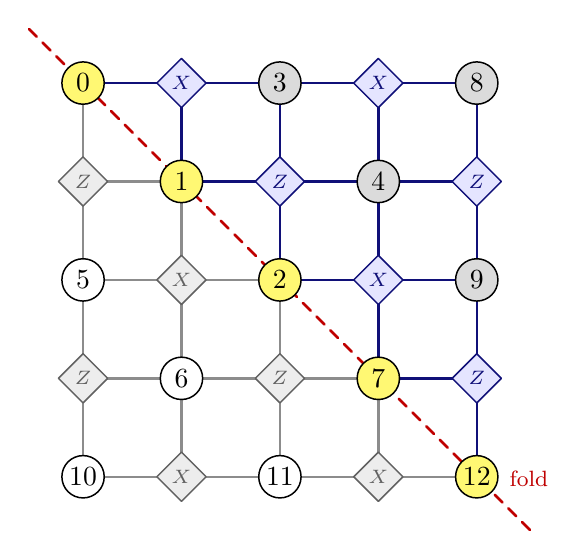
\begin{tikzpicture}[x=1.25cm,y=1.25cm,line cap=round,line join=round]
\draw[botline,line width=0.9pt] (0,-1) -- (1,-1);
\draw[botline,line width=0.9pt] (0,-1) -- (0,-2);
\draw[botline,line width=0.9pt] (0,-1) -- (0,0);
\draw[botline,line width=0.9pt] (1,-2) -- (2,-2);
\draw[botline,line width=0.9pt] (1,-2) -- (0,-2);
\draw[botline,line width=0.9pt] (1,-2) -- (1,-3);
\draw[botline,line width=0.9pt] (1,-2) -- (1,-1);
\draw[botline,line width=0.9pt] (0,-3) -- (1,-3);
\draw[botline,line width=0.9pt] (0,-3) -- (0,-4);
\draw[botline,line width=0.9pt] (0,-3) -- (0,-2);
\draw[botline,line width=0.9pt] (2,-3) -- (3,-3);
\draw[botline,line width=0.9pt] (2,-3) -- (1,-3);
\draw[botline,line width=0.9pt] (2,-3) -- (2,-4);
\draw[botline,line width=0.9pt] (2,-3) -- (2,-2);
\draw[botline,line width=0.9pt] (1,-4) -- (2,-4);
\draw[botline,line width=0.9pt] (1,-4) -- (0,-4);
\draw[botline,line width=0.9pt] (1,-4) -- (1,-3);
\draw[botline,line width=0.9pt] (3,-4) -- (4,-4);
\draw[botline,line width=0.9pt] (3,-4) -- (2,-4);
\draw[botline,line width=0.9pt] (3,-4) -- (3,-3);
\draw[topline,line width=0.9pt] (1,0) -- (2,0);
\draw[topline,line width=0.9pt] (1,0) -- (0,0);
\draw[topline,line width=0.9pt] (1,0) -- (1,-1);
\draw[topline,line width=0.9pt] (2,-1) -- (3,-1);
\draw[topline,line width=0.9pt] (2,-1) -- (1,-1);
\draw[topline,line width=0.9pt] (2,-1) -- (2,-2);
\draw[topline,line width=0.9pt] (2,-1) -- (2,0);
\draw[topline,line width=0.9pt] (3,0) -- (4,0);
\draw[topline,line width=0.9pt] (3,0) -- (2,0);
\draw[topline,line width=0.9pt] (3,0) -- (3,-1);
\draw[topline,line width=0.9pt] (3,-2) -- (4,-2);
\draw[topline,line width=0.9pt] (3,-2) -- (2,-2);
\draw[topline,line width=0.9pt] (3,-2) -- (3,-3);
\draw[topline,line width=0.9pt] (3,-2) -- (3,-1);
\draw[topline,line width=0.9pt] (4,-1) -- (3,-1);
\draw[topline,line width=0.9pt] (4,-1) -- (4,-2);
\draw[topline,line width=0.9pt] (4,-1) -- (4,0);
\draw[topline,line width=0.9pt] (4,-3) -- (3,-3);
\draw[topline,line width=0.9pt] (4,-3) -- (4,-4);
\draw[topline,line width=0.9pt] (4,-3) -- (4,-2);
\draw[foldline] (-0.55,0.55) -- (4.55,-4.55);
\node[foldtext,anchor=south west,inner sep=1pt] at (4.3,-4.13) {fold};
\draw[botanc,line width=0.54pt] (-0.25,-1) -- (0,-0.75) -- (0.25,-1) -- (0,-1.25) -- cycle;
\node[anclabel,botanctext] at (0,-1) {\scriptsize $Z$};
\draw[botanc,line width=0.54pt] (0.75,-2) -- (1,-1.75) -- (1.25,-2) -- (1,-2.25) -- cycle;
\node[anclabel,botanctext] at (1,-2) {\scriptsize $X$};
\draw[botanc,line width=0.54pt] (-0.25,-3) -- (0,-2.75) -- (0.25,-3) -- (0,-3.25) -- cycle;
\node[anclabel,botanctext] at (0,-3) {\scriptsize $Z$};
\draw[botanc,line width=0.54pt] (1.75,-3) -- (2,-2.75) -- (2.25,-3) -- (2,-3.25) -- cycle;
\node[anclabel,botanctext] at (2,-3) {\scriptsize $Z$};
\draw[botanc,line width=0.54pt] (0.75,-4) -- (1,-3.75) -- (1.25,-4) -- (1,-4.25) -- cycle;
\node[anclabel,botanctext] at (1,-4) {\scriptsize $X$};
\draw[botanc,line width=0.54pt] (2.75,-4) -- (3,-3.75) -- (3.25,-4) -- (3,-4.25) -- cycle;
\node[anclabel,botanctext] at (3,-4) {\scriptsize $X$};
\draw[topanc,line width=0.54pt] (0.75,0) -- (1,0.25) -- (1.25,0) -- (1,-0.25) -- cycle;
\node[anclabel,topanctext] at (1,0) {\scriptsize $X$};
\draw[topanc,line width=0.54pt] (1.75,-1) -- (2,-0.75) -- (2.25,-1) -- (2,-1.25) -- cycle;
\node[anclabel,topanctext] at (2,-1) {\scriptsize $Z$};
\draw[topanc,line width=0.54pt] (2.75,0) -- (3,0.25) -- (3.25,0) -- (3,-0.25) -- cycle;
\node[anclabel,topanctext] at (3,0) {\scriptsize $X$};
\draw[topanc,line width=0.54pt] (2.75,-2) -- (3,-1.75) -- (3.25,-2) -- (3,-2.25) -- cycle;
\node[anclabel,topanctext] at (3,-2) {\scriptsize $X$};
\draw[topanc,line width=0.54pt] (3.75,-1) -- (4,-0.75) -- (4.25,-1) -- (4,-1.25) -- cycle;
\node[anclabel,topanctext] at (4,-1) {\scriptsize $Z$};
\draw[topanc,line width=0.54pt] (3.75,-3) -- (4,-2.75) -- (4.25,-3) -- (4,-3.25) -- cycle;
\node[anclabel,topanctext] at (4,-3) {\scriptsize $Z$};
\draw[foldq,line width=0.54pt] (0,0) circle[radius=0.215];
\node[qlabel] at (0,0) {\normalsize 0};
\draw[foldq,line width=0.54pt] (1,-1) circle[radius=0.215];
\node[qlabel] at (1,-1) {\normalsize 1};
\draw[foldq,line width=0.54pt] (2,-2) circle[radius=0.215];
\node[qlabel] at (2,-2) {\normalsize 2};
\draw[topq,line width=0.54pt] (2,0) circle[radius=0.215];
\node[qlabel] at (2,0) {\normalsize 3};
\draw[topq,line width=0.54pt] (3,-1) circle[radius=0.215];
\node[qlabel] at (3,-1) {\normalsize 4};
\draw[botq,line width=0.54pt] (0,-2) circle[radius=0.215];
\node[qlabel] at (0,-2) {\normalsize 5};
\draw[botq,line width=0.54pt] (1,-3) circle[radius=0.215];
\node[qlabel] at (1,-3) {\normalsize 6};
\draw[foldq,line width=0.54pt] (3,-3) circle[radius=0.215];
\node[qlabel] at (3,-3) {\normalsize 7};
\draw[topq,line width=0.54pt] (4,0) circle[radius=0.215];
\node[qlabel] at (4,0) {\normalsize 8};
\draw[topq,line width=0.54pt] (4,-2) circle[radius=0.215];
\node[qlabel] at (4,-2) {\normalsize 9};
\draw[botq,line width=0.54pt] (0,-4) circle[radius=0.215];
\node[qlabel] at (0,-4) {\normalsize 10};
\draw[botq,line width=0.54pt] (2,-4) circle[radius=0.215];
\node[qlabel] at (2,-4) {\normalsize 11};
\draw[foldq,line width=0.54pt] (4,-4) circle[radius=0.215];
\node[qlabel] at (4,-4) {\normalsize 12};
\end{tikzpicture}

\caption{}
\end{subfigure}\hfill
\begin{subfigure}[b]{0.55\textwidth}
\centering
%% generated by gen_layout.py -- do not edit by hand

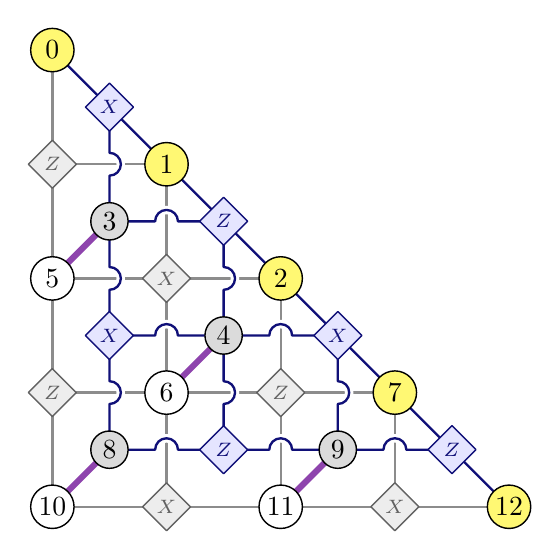
\begin{tikzpicture}[x=1.45cm,y=1.45cm,line cap=round,line join=round]
\draw[botline,line width=0.85pt] (0,-1) -- (0,-0);
\draw[botline,line width=0.85pt] (0,-1) -- (1,-1);
\draw[botline,line width=0.85pt] (0,-1) -- (0,-2);
\draw[botline,line width=0.85pt] (1,-2) -- (1,-1);
\draw[botline,line width=0.85pt] (1,-2) -- (2,-2);
\draw[botline,line width=0.85pt] (1,-2) -- (0,-2);
\draw[botline,line width=0.85pt] (1,-2) -- (1,-3);
\draw[botline,line width=0.85pt] (0,-3) -- (0,-2);
\draw[botline,line width=0.85pt] (0,-3) -- (1,-3);
\draw[botline,line width=0.85pt] (0,-3) -- (0,-4);
\draw[botline,line width=0.85pt] (2,-3) -- (2,-2);
\draw[botline,line width=0.85pt] (2,-3) -- (1,-3);
\draw[botline,line width=0.85pt] (2,-3) -- (3,-3);
\draw[botline,line width=0.85pt] (2,-3) -- (2,-4);
\draw[botline,line width=0.85pt] (1,-4) -- (1,-3);
\draw[botline,line width=0.85pt] (1,-4) -- (0,-4);
\draw[botline,line width=0.85pt] (1,-4) -- (2,-4);
\draw[botline,line width=0.85pt] (3,-4) -- (3,-3);
\draw[botline,line width=0.85pt] (3,-4) -- (2,-4);
\draw[botline,line width=0.85pt] (3,-4) -- (4,-4);
\draw[pairline,line width=2.21pt] (0,-2) -- (0.5,-1.5);
\draw[pairline,line width=2.21pt] (1,-3) -- (1.5,-2.5);
\draw[pairline,line width=2.21pt] (0,-4) -- (0.5,-3.5);
\draw[pairline,line width=2.21pt] (2,-4) -- (2.5,-3.5);
\draw[topline,line width=0.85pt] (0.5,-0.5) -- (0,-0);
\draw[topline,line width=0.85pt] (0.5,-0.5) -- (1,-1);
\draw[white,line width=3.05pt,line cap=butt] (0.5,-0.9) arc[start angle=90,end angle=-90,radius=0.1];
\draw[topline,line width=0.85pt] (0.5,-0.5) -- (0.5,-0.9) arc[start angle=90,end angle=-90,radius=0.1] -- (0.5,-1.5);
\draw[topline,line width=0.85pt] (1.5,-1.5) -- (1,-1);
\draw[topline,line width=0.85pt] (1.5,-1.5) -- (2,-2);
\draw[white,line width=3.05pt,line cap=butt] (0.9,-1.5) arc[start angle=180,end angle=0,radius=0.1];
\draw[topline,line width=0.85pt] (0.5,-1.5) -- (0.9,-1.5) arc[start angle=180,end angle=0,radius=0.1] -- (1.5,-1.5);
\draw[white,line width=3.05pt,line cap=butt] (1.5,-1.9) arc[start angle=90,end angle=-90,radius=0.1];
\draw[topline,line width=0.85pt] (1.5,-1.5) -- (1.5,-1.9) arc[start angle=90,end angle=-90,radius=0.1] -- (1.5,-2.5);
\draw[white,line width=3.05pt,line cap=butt] (0.5,-1.9) arc[start angle=90,end angle=-90,radius=0.1];
\draw[topline,line width=0.85pt] (0.5,-1.5) -- (0.5,-1.9) arc[start angle=90,end angle=-90,radius=0.1] -- (0.5,-2.5);
\draw[white,line width=3.05pt,line cap=butt] (0.9,-2.5) arc[start angle=180,end angle=0,radius=0.1];
\draw[topline,line width=0.85pt] (0.5,-2.5) -- (0.9,-2.5) arc[start angle=180,end angle=0,radius=0.1] -- (1.5,-2.5);
\draw[white,line width=3.05pt,line cap=butt] (0.5,-2.9) arc[start angle=90,end angle=-90,radius=0.1];
\draw[topline,line width=0.85pt] (0.5,-2.5) -- (0.5,-2.9) arc[start angle=90,end angle=-90,radius=0.1] -- (0.5,-3.5);
\draw[topline,line width=0.85pt] (2.5,-2.5) -- (2,-2);
\draw[white,line width=3.05pt,line cap=butt] (1.9,-2.5) arc[start angle=180,end angle=0,radius=0.1];
\draw[topline,line width=0.85pt] (1.5,-2.5) -- (1.9,-2.5) arc[start angle=180,end angle=0,radius=0.1] -- (2.5,-2.5);
\draw[topline,line width=0.85pt] (2.5,-2.5) -- (3,-3);
\draw[white,line width=3.05pt,line cap=butt] (2.5,-2.9) arc[start angle=90,end angle=-90,radius=0.1];
\draw[topline,line width=0.85pt] (2.5,-2.5) -- (2.5,-2.9) arc[start angle=90,end angle=-90,radius=0.1] -- (2.5,-3.5);
\draw[white,line width=3.05pt,line cap=butt] (1.5,-2.9) arc[start angle=90,end angle=-90,radius=0.1];
\draw[topline,line width=0.85pt] (1.5,-2.5) -- (1.5,-2.9) arc[start angle=90,end angle=-90,radius=0.1] -- (1.5,-3.5);
\draw[white,line width=3.05pt,line cap=butt] (0.9,-3.5) arc[start angle=180,end angle=0,radius=0.1];
\draw[topline,line width=0.85pt] (0.5,-3.5) -- (0.9,-3.5) arc[start angle=180,end angle=0,radius=0.1] -- (1.5,-3.5);
\draw[white,line width=3.05pt,line cap=butt] (1.9,-3.5) arc[start angle=180,end angle=0,radius=0.1];
\draw[topline,line width=0.85pt] (1.5,-3.5) -- (1.9,-3.5) arc[start angle=180,end angle=0,radius=0.1] -- (2.5,-3.5);
\draw[topline,line width=0.85pt] (3.5,-3.5) -- (3,-3);
\draw[white,line width=3.05pt,line cap=butt] (2.9,-3.5) arc[start angle=180,end angle=0,radius=0.1];
\draw[topline,line width=0.85pt] (2.5,-3.5) -- (2.9,-3.5) arc[start angle=180,end angle=0,radius=0.1] -- (3.5,-3.5);
\draw[topline,line width=0.85pt] (3.5,-3.5) -- (4,-4);
\draw[botanc,line width=0.51pt] (-0.21,-1) -- (0,-0.79) -- (0.21,-1) -- (0,-1.21) -- cycle;
\node[anclabel,botanctext] at (0,-1) {\scriptsize $Z$};
\draw[botanc,line width=0.51pt] (0.79,-2) -- (1,-1.79) -- (1.21,-2) -- (1,-2.21) -- cycle;
\node[anclabel,botanctext] at (1,-2) {\scriptsize $X$};
\draw[botanc,line width=0.51pt] (-0.21,-3) -- (0,-2.79) -- (0.21,-3) -- (0,-3.21) -- cycle;
\node[anclabel,botanctext] at (0,-3) {\scriptsize $Z$};
\draw[botanc,line width=0.51pt] (1.79,-3) -- (2,-2.79) -- (2.21,-3) -- (2,-3.21) -- cycle;
\node[anclabel,botanctext] at (2,-3) {\scriptsize $Z$};
\draw[botanc,line width=0.51pt] (0.79,-4) -- (1,-3.79) -- (1.21,-4) -- (1,-4.21) -- cycle;
\node[anclabel,botanctext] at (1,-4) {\scriptsize $X$};
\draw[botanc,line width=0.51pt] (2.79,-4) -- (3,-3.79) -- (3.21,-4) -- (3,-4.21) -- cycle;
\node[anclabel,botanctext] at (3,-4) {\scriptsize $X$};
\draw[topanc,line width=0.51pt] (0.29,-0.5) -- (0.5,-0.29) -- (0.71,-0.5) -- (0.5,-0.71) -- cycle;
\node[anclabel,topanctext] at (0.5,-0.5) {\scriptsize $X$};
\draw[topanc,line width=0.51pt] (1.29,-1.5) -- (1.5,-1.29) -- (1.71,-1.5) -- (1.5,-1.71) -- cycle;
\node[anclabel,topanctext] at (1.5,-1.5) {\scriptsize $Z$};
\draw[topanc,line width=0.51pt] (0.29,-2.5) -- (0.5,-2.29) -- (0.71,-2.5) -- (0.5,-2.71) -- cycle;
\node[anclabel,topanctext] at (0.5,-2.5) {\scriptsize $X$};
\draw[topanc,line width=0.51pt] (2.29,-2.5) -- (2.5,-2.29) -- (2.71,-2.5) -- (2.5,-2.71) -- cycle;
\node[anclabel,topanctext] at (2.5,-2.5) {\scriptsize $X$};
\draw[topanc,line width=0.51pt] (1.29,-3.5) -- (1.5,-3.29) -- (1.71,-3.5) -- (1.5,-3.71) -- cycle;
\node[anclabel,topanctext] at (1.5,-3.5) {\scriptsize $Z$};
\draw[topanc,line width=0.51pt] (3.29,-3.5) -- (3.5,-3.29) -- (3.71,-3.5) -- (3.5,-3.71) -- cycle;
\node[anclabel,topanctext] at (3.5,-3.5) {\scriptsize $Z$};
\draw[foldq,line width=0.51pt] (0,-0) circle[radius=0.19];
\node[qlabel] at (0,-0) {\normalsize 0};
\draw[foldq,line width=0.51pt] (1,-1) circle[radius=0.19];
\node[qlabel] at (1,-1) {\normalsize 1};
\draw[foldq,line width=0.51pt] (2,-2) circle[radius=0.19];
\node[qlabel] at (2,-2) {\normalsize 2};
\draw[topq,line width=0.51pt] (0.5,-1.5) circle[radius=0.1634];
\node[qlabel] at (0.5,-1.5) {\normalsize 3};
\draw[topq,line width=0.51pt] (1.5,-2.5) circle[radius=0.1634];
\node[qlabel] at (1.5,-2.5) {\normalsize 4};
\draw[botq,line width=0.51pt] (0,-2) circle[radius=0.19];
\node[qlabel] at (0,-2) {\normalsize 5};
\draw[botq,line width=0.51pt] (1,-3) circle[radius=0.19];
\node[qlabel] at (1,-3) {\normalsize 6};
\draw[foldq,line width=0.51pt] (3,-3) circle[radius=0.19];
\node[qlabel] at (3,-3) {\normalsize 7};
\draw[topq,line width=0.51pt] (0.5,-3.5) circle[radius=0.1634];
\node[qlabel] at (0.5,-3.5) {\normalsize 8};
\draw[topq,line width=0.51pt] (2.5,-3.5) circle[radius=0.1634];
\node[qlabel] at (2.5,-3.5) {\normalsize 9};
\draw[botq,line width=0.51pt] (0,-4) circle[radius=0.19];
\node[qlabel] at (0,-4) {\normalsize 10};
\draw[botq,line width=0.51pt] (2,-4) circle[radius=0.19];
\node[qlabel] at (2,-4) {\normalsize 11};
\draw[foldq,line width=0.51pt] (4,-4) circle[radius=0.19];
\node[qlabel] at (4,-4) {\normalsize 12};
\end{tikzpicture}

\caption{}
\end{subfigure}
\caption{The distance-3 code, 13 data qubits (circles) and 12 check ancillas (diamonds, marked
with the type of check they measure). (a)~The unfolded patch. The dashed line is the fold. The
half below it, drawn in grey, becomes the bottom layer, and the half above it, drawn in blue,
becomes the top layer. (b)~The layout. Yellow circles are the fold qubits, white circles the
bottom-layer data qubits and grey circles the top-layer data qubits. Grey lines are bottom-layer
couplers, blue lines are top-layer couplers, and a blue line hops over a grey line at each of
the 12 crossovers. Each purple line couples the two data qubits of a pair, 3--5, 4--6, 8--10
and 9--11.}
\label{fig:d3}
\end{figure}

\section{The layout}

Fold the patch along the diagonal and keep both halves in the plane.

\begin{enumerate}
\item \textbf{Bottom layer.} The half $x\le y$ stays where it is. It holds the fold qubits,
$(d-1)^2$ data qubits and $d(d-1)$ ancillas on a square lattice of pitch $a$, and a coupler of
length $a$ joins each ancilla to each of its neighbours.
\item \textbf{Top layer.} The mirror image of the half $x>y$ falls on the same sites. Shift it
by half a cell towards the fold, so that the image of $(y,x)$ sits at
$(x+\tfrac12,\;y-\tfrac12)$, the centre of a cell of the bottom layer. The top layer is again a
square lattice of pitch $a$ with couplers of length $a$.
\item \textbf{Fold.} The fold qubits exist once and belong to both layers. The $2d-2$ top-layer
ancillas next to the fold land on the hypotenuse, midway between two fold qubits, and couple to
both with couplers of length $a/\sqrt2$.
\item \textbf{Pairs.} The partner of the bottom-layer data qubit at $(x,y)$ sits at
$(x+\tfrac12,\;y-\tfrac12)$, a distance $a/\sqrt2$ away along the diagonal of the cell. One
coupler joins the two.
\item \textbf{Crossovers.} A top-layer coupler of length $a$ runs from one cell centre to the
next and crosses the bottom-layer coupler on the edge between the two cells. The two meet at
right angles, each at its midpoint. Nothing else crosses, because the pair couplers and the couplers
at the fold stay inside one cell.
\end{enumerate}

\paragraph{Comparison with Moussa's planar layout.} Moussa~\cite{Moussa2016} also puts the folded
code in one plane, on a lattice where every site holds one qudit of each half. There the check
circuits need two-qudit gates between qudits that are not neighbours. With nearest-neighbour gates
only, every round needs one pairwise swap of all top and bottom qudits, which also spreads errors
between the halves, and an extra $\mathrm{CX}^\dagger$ between two ancillas next to the fold;
turning an ordinary patch into the folded one by local swaps takes depth $6d-5$. Here each half
keeps its own ancillas and couplers, so a check round is the ordinary one with no swaps. The price
is the $2(d-1)(2d-3)$ crossovers.

Figure~\ref{fig:tile} shows the cells from which every distance is built. In the bulk, the
centre of a cell holds a top-layer element of the same kind as the bottom-left corner of the
cell. Over a data qubit sits its partner, with the pair coupler between them. Over an ancilla
sits an ancilla, and no coupler joins these two. A cell on the fold differs in two ways. Its
fourth corner is empty, and the ancilla at its centre couples to the two fold qubits on its
corners.

\begin{figure}[t]
\centering
%% generated by gen_layout.py -- do not edit by hand

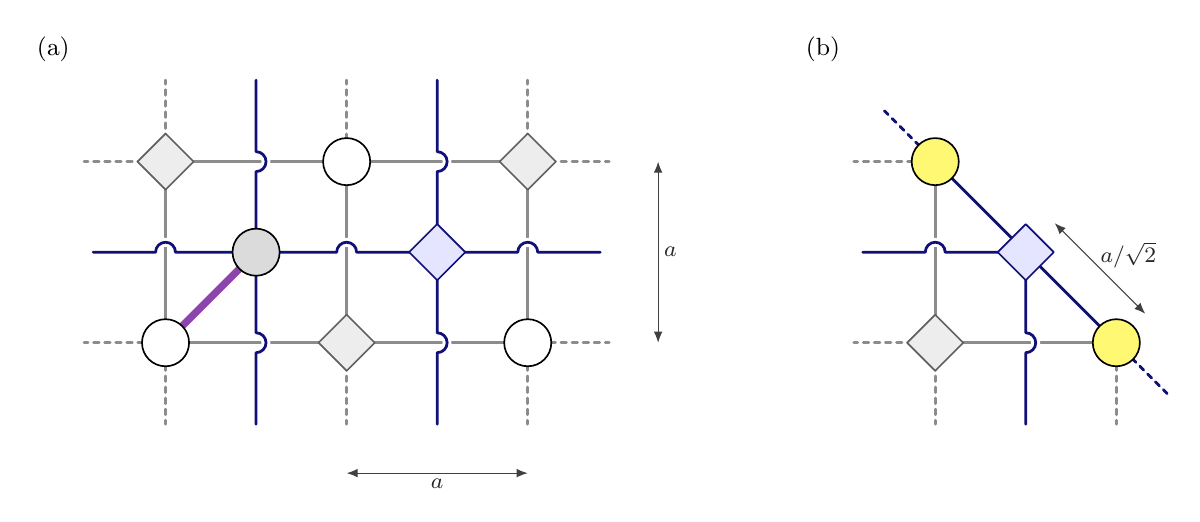
\begin{tikzpicture}[x=2.3cm,y=2.3cm,line cap=round,line join=round]
\begin{scope}
\node[panel] at (-0.62,0.62) {(a)};
\draw[botline,line width=1pt] (0,0) -- (1,0);
\draw[botline,line width=1pt] (1,0) -- (2,0);
\draw[botline,line width=1pt] (0,-1) -- (1,-1);
\draw[botline,line width=1pt] (1,-1) -- (2,-1);
\draw[botline,line width=1pt] (0,0) -- (0,-1);
\draw[botline,line width=1pt] (1,0) -- (1,-1);
\draw[botline,line width=1pt] (2,0) -- (2,-1);
\draw[botline,line width=1pt,dash pattern=on 2pt off 2pt] (0,0) -- (-0.45,0);
\draw[botline,line width=1pt,dash pattern=on 2pt off 2pt] (0,-1) -- (-0.45,-1);
\draw[botline,line width=1pt,dash pattern=on 2pt off 2pt] (2,0) -- (2.45,0);
\draw[botline,line width=1pt,dash pattern=on 2pt off 2pt] (2,-1) -- (2.45,-1);
\draw[botline,line width=1pt,dash pattern=on 2pt off 2pt] (0,0) -- (0,0.45);
\draw[botline,line width=1pt,dash pattern=on 2pt off 2pt] (1,0) -- (1,0.45);
\draw[botline,line width=1pt,dash pattern=on 2pt off 2pt] (2,0) -- (2,0.45);
\draw[botline,line width=1pt,dash pattern=on 2pt off 2pt] (0,-1) -- (0,-1.45);
\draw[botline,line width=1pt,dash pattern=on 2pt off 2pt] (1,-1) -- (1,-1.45);
\draw[botline,line width=1pt,dash pattern=on 2pt off 2pt] (2,-1) -- (2,-1.45);
\draw[pairline,line width=2.6pt] (0,-1) -- (0.5,-0.5);
\draw[white,line width=3.2pt,line cap=butt] (0.945,-0.5) arc[start angle=180,end angle=0,radius=0.055];
\draw[topline,line width=1pt] (0.5,-0.5) -- (0.945,-0.5) arc[start angle=180,end angle=0,radius=0.055] -- (1.5,-0.5);
\draw[white,line width=3.2pt,line cap=butt] (0.5,0.055) arc[start angle=90,end angle=-90,radius=0.055];
\draw[topline,line width=1pt] (0.5,0.45) -- (0.5,0.055) arc[start angle=90,end angle=-90,radius=0.055] -- (0.5,-0.5);
\draw[white,line width=3.2pt,line cap=butt] (0.5,-0.945) arc[start angle=90,end angle=-90,radius=0.055];
\draw[topline,line width=1pt] (0.5,-0.5) -- (0.5,-0.945) arc[start angle=90,end angle=-90,radius=0.055] -- (0.5,-1.45);
\draw[white,line width=3.2pt,line cap=butt] (1.5,0.055) arc[start angle=90,end angle=-90,radius=0.055];
\draw[topline,line width=1pt] (1.5,0.45) -- (1.5,0.055) arc[start angle=90,end angle=-90,radius=0.055] -- (1.5,-0.5);
\draw[white,line width=3.2pt,line cap=butt] (1.5,-0.945) arc[start angle=90,end angle=-90,radius=0.055];
\draw[topline,line width=1pt] (1.5,-0.5) -- (1.5,-0.945) arc[start angle=90,end angle=-90,radius=0.055] -- (1.5,-1.45);
\draw[white,line width=3.2pt,line cap=butt] (-0.055,-0.5) arc[start angle=180,end angle=0,radius=0.055];
\draw[topline,line width=1pt] (-0.4,-0.5) -- (-0.055,-0.5) arc[start angle=180,end angle=0,radius=0.055] -- (0.5,-0.5);
\draw[white,line width=3.2pt,line cap=butt] (1.945,-0.5) arc[start angle=180,end angle=0,radius=0.055];
\draw[topline,line width=1pt] (1.5,-0.5) -- (1.945,-0.5) arc[start angle=180,end angle=0,radius=0.055] -- (2.4,-0.5);
\draw[botq,line width=0.6pt] (0,-1) circle[radius=0.13];
\draw[botanc,line width=0.6pt] (0.845,-1) -- (1,-0.845) -- (1.155,-1) -- (1,-1.155) -- cycle;
\draw[botq,line width=0.6pt] (2,-1) circle[radius=0.13];
\draw[botanc,line width=0.6pt] (-0.155,0) -- (0,0.155) -- (0.155,0) -- (0,-0.155) -- cycle;
\draw[botq,line width=0.6pt] (1,0) circle[radius=0.13];
\draw[botanc,line width=0.6pt] (1.845,0) -- (2,0.155) -- (2.155,0) -- (2,-0.155) -- cycle;
\draw[topq,line width=0.6pt] (0.5,-0.5) circle[radius=0.13];
\draw[topanc,line width=0.6pt] (1.345,-0.5) -- (1.5,-0.345) -- (1.655,-0.5) -- (1.5,-0.655) -- cycle;
\draw[dim] (1,-1.72) -- (2,-1.72) node[midway,below,dimtext] {$a$};
\draw[dim] (2.72,0) -- (2.72,-1) node[midway,right,dimtext] {$a$};
\end{scope}
\begin{scope}[shift={(4.25,0)}]
\node[panel] at (-0.62,0.62) {(b)};
\draw[botline,line width=1pt] (0,0) -- (0,-1) -- (1,-1);
\draw[botline,line width=1pt,dash pattern=on 2pt off 2pt] (0,-1) -- (-0.45,-1);
\draw[botline,line width=1pt,dash pattern=on 2pt off 2pt] (0,-1) -- (0,-1.45);
\draw[botline,line width=1pt,dash pattern=on 2pt off 2pt] (1,-1) -- (1,-1.45);
\draw[botline,line width=1pt,dash pattern=on 2pt off 2pt] (0,0) -- (-0.45,0);
\draw[topline,line width=1pt] (0,0) -- (0.5,-0.5) -- (1,-1);
\draw[topline,line width=1pt,dash pattern=on 2pt off 2pt] (0,0) -- (-0.3,0.3);
\draw[topline,line width=1pt,dash pattern=on 2pt off 2pt] (1,-1) -- (1.3,-1.3);
\draw[white,line width=3.2pt,line cap=butt] (-0.055,-0.5) arc[start angle=180,end angle=0,radius=0.055];
\draw[topline,line width=1pt] (-0.4,-0.5) -- (-0.055,-0.5) arc[start angle=180,end angle=0,radius=0.055] -- (0.5,-0.5);
\draw[white,line width=3.2pt,line cap=butt] (0.5,-0.945) arc[start angle=90,end angle=-90,radius=0.055];
\draw[topline,line width=1pt] (0.5,-0.5) -- (0.5,-0.945) arc[start angle=90,end angle=-90,radius=0.055] -- (0.5,-1.45);
\draw[foldq,line width=0.6pt] (0,0) circle[radius=0.13];
\draw[foldq,line width=0.6pt] (1,-1) circle[radius=0.13];
\draw[botanc,line width=0.6pt] (-0.155,-1) -- (0,-0.845) -- (0.155,-1) -- (0,-1.155) -- cycle;
\draw[topanc,line width=0.6pt] (0.345,-0.5) -- (0.5,-0.345) -- (0.655,-0.5) -- (0.5,-0.655) -- cycle;
\draw[dim] (0.66,-0.34) -- (1.16,-0.84) node[midway,above right=-2pt,dimtext] {$a/\sqrt2$};
\end{scope}
\end{tikzpicture}

\caption{The repeating cells. (a)~Two cells of the bulk. The bottom layer (grey lines) puts data
qubits and ancillas alternately on the corners. The top layer (blue lines) puts them on the cell
centres, and each of its couplers hops over one bottom-layer coupler. The purple pair coupler
has length $a/\sqrt2$, half the diagonal of a cell, and every other coupler in the panel has
length $a$. Dashed grey stubs and
the blue lines that leave the panel continue into the neighbouring cells. (b)~A cell on the fold. The two fold qubits (yellow) belong to both
layers. The top-layer ancilla sits between them and couples to each with a coupler of length
$a/\sqrt2$.}
\label{fig:tile}
\end{figure}

\section{Scaling with the distance}

Table~\ref{tab:counts} gives the contents of the layout and Fig.~\ref{fig:family} shows the
first four members at one scale. The layout holds the $(2d-1)^2$ qubits of the unfolded patch on
half the area, a right triangle with legs $(2d-2)\,a$. Growing the distance by one adds two rows
at the bottom of the triangle. Nothing above them moves, and the old bottom edge gains the
couplers that reach into the new rows. A chip built for distance $d$ therefore also runs every
smaller distance on a corner of itself; \texttt{dorito-chip.pdf} outlines the distance-2 and
distance-3 codes on the distance-5 chip.

\begin{table}[!ht]
\centering
\begin{tabular}{@{}lcrrrrr@{}}
\toprule
 & distance $d$ & $d=2$ & $3$ & $4$ & $5$ & $6$\\
\midrule
data qubits & $2d^2-2d+1$ & 5 & 13 & 25 & 41 & 61\\
\quad of which fold qubits & $2d-1$ & 3 & 5 & 7 & 9 & 11\\
\quad pairs & $(d-1)^2$ & 1 & 4 & 9 & 16 & 25\\
check ancillas & $2d(d-1)$ & 4 & 12 & 24 & 40 & 60\\
all qubits & $(2d-1)^2$ & 9 & 25 & 49 & 81 & 121\\
\midrule
couplers, ancilla to data & $4(2d-1)(d-1)$ & 12 & 40 & 84 & 144 & 220\\
\quad of which length $a/\sqrt2$, at the fold & $4(d-1)$ & 4 & 8 & 12 & 16 & 20\\
pair couplers, length $a/\sqrt2$ & $(d-1)^2$ & 1 & 4 & 9 & 16 & 25\\
all couplers & $(d-1)(9d-5)$ & 13 & 44 & 93 & 160 & 245\\
crossovers & $2(d-1)(2d-3)$ & 2 & 12 & 30 & 56 & 90\\
\midrule
most couplers on one data qubit & & 4 & 5 & 5 & 5 & 5\\
most couplers on one ancilla & & 3 & 4 & 4 & 4 & 4\\
leg of the triangle & $(2d-2)\,a$ & $2a$ & $4a$ & $6a$ & $8a$ & $10a$\\
\bottomrule
\end{tabular}
\caption{Contents of the layout. The script \texttt{gen\_layout.py} counted the qubits,
couplers and crossovers and checked each count against its formula.}
\label{tab:counts}
\end{table}

The number of crossovers grows like $4d^2$, which is one per qubit at large $d$. Some crossovers
cannot be avoided. With the pair couplers the coupling graph of $d=3$ is non-planar, and every
larger distance contains it, so for $d\ge3$ no placement in one plane is free of crossings.
At $d=2$ the graph is planar, so another placement could remove the two crossovers of this one.
Whether $2(d-1)(2d-3)$ is the smallest possible number for $d\ge3$ is open.

\begin{figure}[!t]
\centering
\begin{minipage}[b]{0.17\textwidth}\centering %% generated by gen_layout.py -- do not edit by hand

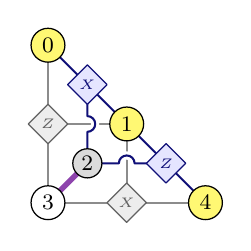
\begin{tikzpicture}[x=1cm,y=1cm,line cap=round,line join=round]
\draw[botline,line width=0.75pt] (0,-1) -- (0,-0);
\draw[botline,line width=0.75pt] (0,-1) -- (1,-1);
\draw[botline,line width=0.75pt] (0,-1) -- (0,-2);
\draw[botline,line width=0.75pt] (1,-2) -- (1,-1);
\draw[botline,line width=0.75pt] (1,-2) -- (0,-2);
\draw[botline,line width=0.75pt] (1,-2) -- (2,-2);
\draw[pairline,line width=1.95pt] (0,-2) -- (0.5,-1.5);
\draw[topline,line width=0.75pt] (0.5,-0.5) -- (0,-0);
\draw[topline,line width=0.75pt] (0.5,-0.5) -- (1,-1);
\draw[white,line width=2.95pt,line cap=butt] (0.5,-0.9) arc[start angle=90,end angle=-90,radius=0.1];
\draw[topline,line width=0.75pt] (0.5,-0.5) -- (0.5,-0.9) arc[start angle=90,end angle=-90,radius=0.1] -- (0.5,-1.5);
\draw[topline,line width=0.75pt] (1.5,-1.5) -- (1,-1);
\draw[white,line width=2.95pt,line cap=butt] (0.9,-1.5) arc[start angle=180,end angle=0,radius=0.1];
\draw[topline,line width=0.75pt] (0.5,-1.5) -- (0.9,-1.5) arc[start angle=180,end angle=0,radius=0.1] -- (1.5,-1.5);
\draw[topline,line width=0.75pt] (1.5,-1.5) -- (2,-2);
\draw[botanc,line width=0.45pt] (-0.25,-1) -- (0,-0.75) -- (0.25,-1) -- (0,-1.25) -- cycle;
\node[anclabel,botanctext] at (0,-1) {\tiny $Z$};
\draw[botanc,line width=0.45pt] (0.75,-2) -- (1,-1.75) -- (1.25,-2) -- (1,-2.25) -- cycle;
\node[anclabel,botanctext] at (1,-2) {\tiny $X$};
\draw[topanc,line width=0.45pt] (0.25,-0.5) -- (0.5,-0.25) -- (0.75,-0.5) -- (0.5,-0.75) -- cycle;
\node[anclabel,topanctext] at (0.5,-0.5) {\tiny $X$};
\draw[topanc,line width=0.45pt] (1.25,-1.5) -- (1.5,-1.25) -- (1.75,-1.5) -- (1.5,-1.75) -- cycle;
\node[anclabel,topanctext] at (1.5,-1.5) {\tiny $Z$};
\draw[foldq,line width=0.45pt] (0,-0) circle[radius=0.215];
\node[qlabel] at (0,-0) {\footnotesize 0};
\draw[foldq,line width=0.45pt] (1,-1) circle[radius=0.215];
\node[qlabel] at (1,-1) {\footnotesize 1};
\draw[topq,line width=0.45pt] (0.5,-1.5) circle[radius=0.1849];
\node[qlabel] at (0.5,-1.5) {\footnotesize 2};
\draw[botq,line width=0.45pt] (0,-2) circle[radius=0.215];
\node[qlabel] at (0,-2) {\footnotesize 3};
\draw[foldq,line width=0.45pt] (2,-2) circle[radius=0.215];
\node[qlabel] at (2,-2) {\footnotesize 4};
\end{tikzpicture}
\\[2pt] {\small $d=2$}\end{minipage}\hfill
\begin{minipage}[b]{0.30\textwidth}\centering %% generated by gen_layout.py -- do not edit by hand

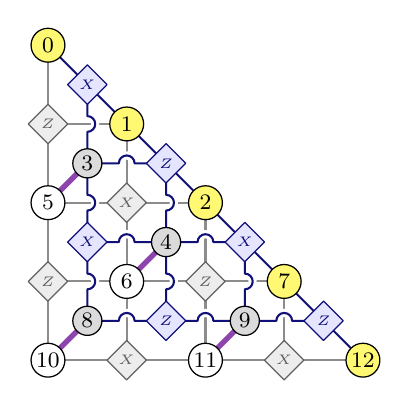
\begin{tikzpicture}[x=1cm,y=1cm,line cap=round,line join=round]
\draw[botline,line width=0.75pt] (0,-1) -- (0,-0);
\draw[botline,line width=0.75pt] (0,-1) -- (1,-1);
\draw[botline,line width=0.75pt] (0,-1) -- (0,-2);
\draw[botline,line width=0.75pt] (1,-2) -- (1,-1);
\draw[botline,line width=0.75pt] (1,-2) -- (2,-2);
\draw[botline,line width=0.75pt] (1,-2) -- (0,-2);
\draw[botline,line width=0.75pt] (1,-2) -- (1,-3);
\draw[botline,line width=0.75pt] (0,-3) -- (0,-2);
\draw[botline,line width=0.75pt] (0,-3) -- (1,-3);
\draw[botline,line width=0.75pt] (0,-3) -- (0,-4);
\draw[botline,line width=0.75pt] (2,-3) -- (2,-2);
\draw[botline,line width=0.75pt] (2,-3) -- (1,-3);
\draw[botline,line width=0.75pt] (2,-3) -- (3,-3);
\draw[botline,line width=0.75pt] (2,-3) -- (2,-4);
\draw[botline,line width=0.75pt] (1,-4) -- (1,-3);
\draw[botline,line width=0.75pt] (1,-4) -- (0,-4);
\draw[botline,line width=0.75pt] (1,-4) -- (2,-4);
\draw[botline,line width=0.75pt] (3,-4) -- (3,-3);
\draw[botline,line width=0.75pt] (3,-4) -- (2,-4);
\draw[botline,line width=0.75pt] (3,-4) -- (4,-4);
\draw[pairline,line width=1.95pt] (0,-2) -- (0.5,-1.5);
\draw[pairline,line width=1.95pt] (1,-3) -- (1.5,-2.5);
\draw[pairline,line width=1.95pt] (0,-4) -- (0.5,-3.5);
\draw[pairline,line width=1.95pt] (2,-4) -- (2.5,-3.5);
\draw[topline,line width=0.75pt] (0.5,-0.5) -- (0,-0);
\draw[topline,line width=0.75pt] (0.5,-0.5) -- (1,-1);
\draw[white,line width=2.95pt,line cap=butt] (0.5,-0.9) arc[start angle=90,end angle=-90,radius=0.1];
\draw[topline,line width=0.75pt] (0.5,-0.5) -- (0.5,-0.9) arc[start angle=90,end angle=-90,radius=0.1] -- (0.5,-1.5);
\draw[topline,line width=0.75pt] (1.5,-1.5) -- (1,-1);
\draw[topline,line width=0.75pt] (1.5,-1.5) -- (2,-2);
\draw[white,line width=2.95pt,line cap=butt] (0.9,-1.5) arc[start angle=180,end angle=0,radius=0.1];
\draw[topline,line width=0.75pt] (0.5,-1.5) -- (0.9,-1.5) arc[start angle=180,end angle=0,radius=0.1] -- (1.5,-1.5);
\draw[white,line width=2.95pt,line cap=butt] (1.5,-1.9) arc[start angle=90,end angle=-90,radius=0.1];
\draw[topline,line width=0.75pt] (1.5,-1.5) -- (1.5,-1.9) arc[start angle=90,end angle=-90,radius=0.1] -- (1.5,-2.5);
\draw[white,line width=2.95pt,line cap=butt] (0.5,-1.9) arc[start angle=90,end angle=-90,radius=0.1];
\draw[topline,line width=0.75pt] (0.5,-1.5) -- (0.5,-1.9) arc[start angle=90,end angle=-90,radius=0.1] -- (0.5,-2.5);
\draw[white,line width=2.95pt,line cap=butt] (0.9,-2.5) arc[start angle=180,end angle=0,radius=0.1];
\draw[topline,line width=0.75pt] (0.5,-2.5) -- (0.9,-2.5) arc[start angle=180,end angle=0,radius=0.1] -- (1.5,-2.5);
\draw[white,line width=2.95pt,line cap=butt] (0.5,-2.9) arc[start angle=90,end angle=-90,radius=0.1];
\draw[topline,line width=0.75pt] (0.5,-2.5) -- (0.5,-2.9) arc[start angle=90,end angle=-90,radius=0.1] -- (0.5,-3.5);
\draw[topline,line width=0.75pt] (2.5,-2.5) -- (2,-2);
\draw[white,line width=2.95pt,line cap=butt] (1.9,-2.5) arc[start angle=180,end angle=0,radius=0.1];
\draw[topline,line width=0.75pt] (1.5,-2.5) -- (1.9,-2.5) arc[start angle=180,end angle=0,radius=0.1] -- (2.5,-2.5);
\draw[topline,line width=0.75pt] (2.5,-2.5) -- (3,-3);
\draw[white,line width=2.95pt,line cap=butt] (2.5,-2.9) arc[start angle=90,end angle=-90,radius=0.1];
\draw[topline,line width=0.75pt] (2.5,-2.5) -- (2.5,-2.9) arc[start angle=90,end angle=-90,radius=0.1] -- (2.5,-3.5);
\draw[white,line width=2.95pt,line cap=butt] (1.5,-2.9) arc[start angle=90,end angle=-90,radius=0.1];
\draw[topline,line width=0.75pt] (1.5,-2.5) -- (1.5,-2.9) arc[start angle=90,end angle=-90,radius=0.1] -- (1.5,-3.5);
\draw[white,line width=2.95pt,line cap=butt] (0.9,-3.5) arc[start angle=180,end angle=0,radius=0.1];
\draw[topline,line width=0.75pt] (0.5,-3.5) -- (0.9,-3.5) arc[start angle=180,end angle=0,radius=0.1] -- (1.5,-3.5);
\draw[white,line width=2.95pt,line cap=butt] (1.9,-3.5) arc[start angle=180,end angle=0,radius=0.1];
\draw[topline,line width=0.75pt] (1.5,-3.5) -- (1.9,-3.5) arc[start angle=180,end angle=0,radius=0.1] -- (2.5,-3.5);
\draw[topline,line width=0.75pt] (3.5,-3.5) -- (3,-3);
\draw[white,line width=2.95pt,line cap=butt] (2.9,-3.5) arc[start angle=180,end angle=0,radius=0.1];
\draw[topline,line width=0.75pt] (2.5,-3.5) -- (2.9,-3.5) arc[start angle=180,end angle=0,radius=0.1] -- (3.5,-3.5);
\draw[topline,line width=0.75pt] (3.5,-3.5) -- (4,-4);
\draw[botanc,line width=0.45pt] (-0.25,-1) -- (0,-0.75) -- (0.25,-1) -- (0,-1.25) -- cycle;
\node[anclabel,botanctext] at (0,-1) {\tiny $Z$};
\draw[botanc,line width=0.45pt] (0.75,-2) -- (1,-1.75) -- (1.25,-2) -- (1,-2.25) -- cycle;
\node[anclabel,botanctext] at (1,-2) {\tiny $X$};
\draw[botanc,line width=0.45pt] (-0.25,-3) -- (0,-2.75) -- (0.25,-3) -- (0,-3.25) -- cycle;
\node[anclabel,botanctext] at (0,-3) {\tiny $Z$};
\draw[botanc,line width=0.45pt] (1.75,-3) -- (2,-2.75) -- (2.25,-3) -- (2,-3.25) -- cycle;
\node[anclabel,botanctext] at (2,-3) {\tiny $Z$};
\draw[botanc,line width=0.45pt] (0.75,-4) -- (1,-3.75) -- (1.25,-4) -- (1,-4.25) -- cycle;
\node[anclabel,botanctext] at (1,-4) {\tiny $X$};
\draw[botanc,line width=0.45pt] (2.75,-4) -- (3,-3.75) -- (3.25,-4) -- (3,-4.25) -- cycle;
\node[anclabel,botanctext] at (3,-4) {\tiny $X$};
\draw[topanc,line width=0.45pt] (0.25,-0.5) -- (0.5,-0.25) -- (0.75,-0.5) -- (0.5,-0.75) -- cycle;
\node[anclabel,topanctext] at (0.5,-0.5) {\tiny $X$};
\draw[topanc,line width=0.45pt] (1.25,-1.5) -- (1.5,-1.25) -- (1.75,-1.5) -- (1.5,-1.75) -- cycle;
\node[anclabel,topanctext] at (1.5,-1.5) {\tiny $Z$};
\draw[topanc,line width=0.45pt] (0.25,-2.5) -- (0.5,-2.25) -- (0.75,-2.5) -- (0.5,-2.75) -- cycle;
\node[anclabel,topanctext] at (0.5,-2.5) {\tiny $X$};
\draw[topanc,line width=0.45pt] (2.25,-2.5) -- (2.5,-2.25) -- (2.75,-2.5) -- (2.5,-2.75) -- cycle;
\node[anclabel,topanctext] at (2.5,-2.5) {\tiny $X$};
\draw[topanc,line width=0.45pt] (1.25,-3.5) -- (1.5,-3.25) -- (1.75,-3.5) -- (1.5,-3.75) -- cycle;
\node[anclabel,topanctext] at (1.5,-3.5) {\tiny $Z$};
\draw[topanc,line width=0.45pt] (3.25,-3.5) -- (3.5,-3.25) -- (3.75,-3.5) -- (3.5,-3.75) -- cycle;
\node[anclabel,topanctext] at (3.5,-3.5) {\tiny $Z$};
\draw[foldq,line width=0.45pt] (0,-0) circle[radius=0.215];
\node[qlabel] at (0,-0) {\footnotesize 0};
\draw[foldq,line width=0.45pt] (1,-1) circle[radius=0.215];
\node[qlabel] at (1,-1) {\footnotesize 1};
\draw[foldq,line width=0.45pt] (2,-2) circle[radius=0.215];
\node[qlabel] at (2,-2) {\footnotesize 2};
\draw[topq,line width=0.45pt] (0.5,-1.5) circle[radius=0.1849];
\node[qlabel] at (0.5,-1.5) {\footnotesize 3};
\draw[topq,line width=0.45pt] (1.5,-2.5) circle[radius=0.1849];
\node[qlabel] at (1.5,-2.5) {\footnotesize 4};
\draw[botq,line width=0.45pt] (0,-2) circle[radius=0.215];
\node[qlabel] at (0,-2) {\footnotesize 5};
\draw[botq,line width=0.45pt] (1,-3) circle[radius=0.215];
\node[qlabel] at (1,-3) {\footnotesize 6};
\draw[foldq,line width=0.45pt] (3,-3) circle[radius=0.215];
\node[qlabel] at (3,-3) {\footnotesize 7};
\draw[topq,line width=0.45pt] (0.5,-3.5) circle[radius=0.1849];
\node[qlabel] at (0.5,-3.5) {\footnotesize 8};
\draw[topq,line width=0.45pt] (2.5,-3.5) circle[radius=0.1849];
\node[qlabel] at (2.5,-3.5) {\footnotesize 9};
\draw[botq,line width=0.45pt] (0,-4) circle[radius=0.215];
\node[qlabel] at (0,-4) {\footnotesize 10};
\draw[botq,line width=0.45pt] (2,-4) circle[radius=0.215];
\node[qlabel] at (2,-4) {\footnotesize 11};
\draw[foldq,line width=0.45pt] (4,-4) circle[radius=0.215];
\node[qlabel] at (4,-4) {\footnotesize 12};
\end{tikzpicture}
\\[2pt] {\small $d=3$}\end{minipage}\hfill
\begin{minipage}[b]{0.44\textwidth}\centering %% generated by gen_layout.py -- do not edit by hand

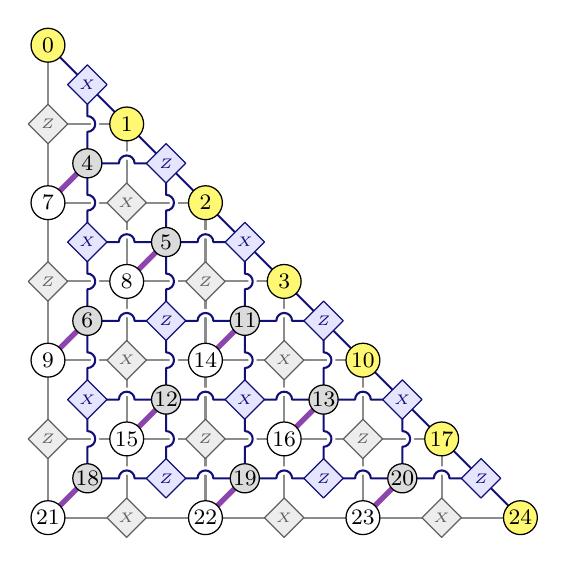
\begin{tikzpicture}[x=1cm,y=1cm,line cap=round,line join=round]
\draw[botline,line width=0.75pt] (0,-1) -- (0,-0);
\draw[botline,line width=0.75pt] (0,-1) -- (1,-1);
\draw[botline,line width=0.75pt] (0,-1) -- (0,-2);
\draw[botline,line width=0.75pt] (1,-2) -- (1,-1);
\draw[botline,line width=0.75pt] (1,-2) -- (2,-2);
\draw[botline,line width=0.75pt] (1,-2) -- (0,-2);
\draw[botline,line width=0.75pt] (1,-2) -- (1,-3);
\draw[botline,line width=0.75pt] (0,-3) -- (0,-2);
\draw[botline,line width=0.75pt] (0,-3) -- (1,-3);
\draw[botline,line width=0.75pt] (0,-3) -- (0,-4);
\draw[botline,line width=0.75pt] (2,-3) -- (2,-2);
\draw[botline,line width=0.75pt] (2,-3) -- (3,-3);
\draw[botline,line width=0.75pt] (2,-3) -- (1,-3);
\draw[botline,line width=0.75pt] (2,-3) -- (2,-4);
\draw[botline,line width=0.75pt] (1,-4) -- (1,-3);
\draw[botline,line width=0.75pt] (1,-4) -- (0,-4);
\draw[botline,line width=0.75pt] (1,-4) -- (2,-4);
\draw[botline,line width=0.75pt] (1,-4) -- (1,-5);
\draw[botline,line width=0.75pt] (3,-4) -- (3,-3);
\draw[botline,line width=0.75pt] (3,-4) -- (4,-4);
\draw[botline,line width=0.75pt] (3,-4) -- (2,-4);
\draw[botline,line width=0.75pt] (3,-4) -- (3,-5);
\draw[botline,line width=0.75pt] (0,-5) -- (0,-4);
\draw[botline,line width=0.75pt] (0,-5) -- (1,-5);
\draw[botline,line width=0.75pt] (0,-5) -- (0,-6);
\draw[botline,line width=0.75pt] (2,-5) -- (2,-4);
\draw[botline,line width=0.75pt] (2,-5) -- (1,-5);
\draw[botline,line width=0.75pt] (2,-5) -- (3,-5);
\draw[botline,line width=0.75pt] (2,-5) -- (2,-6);
\draw[botline,line width=0.75pt] (4,-5) -- (4,-4);
\draw[botline,line width=0.75pt] (4,-5) -- (3,-5);
\draw[botline,line width=0.75pt] (4,-5) -- (5,-5);
\draw[botline,line width=0.75pt] (4,-5) -- (4,-6);
\draw[botline,line width=0.75pt] (1,-6) -- (1,-5);
\draw[botline,line width=0.75pt] (1,-6) -- (0,-6);
\draw[botline,line width=0.75pt] (1,-6) -- (2,-6);
\draw[botline,line width=0.75pt] (3,-6) -- (3,-5);
\draw[botline,line width=0.75pt] (3,-6) -- (2,-6);
\draw[botline,line width=0.75pt] (3,-6) -- (4,-6);
\draw[botline,line width=0.75pt] (5,-6) -- (5,-5);
\draw[botline,line width=0.75pt] (5,-6) -- (4,-6);
\draw[botline,line width=0.75pt] (5,-6) -- (6,-6);
\draw[pairline,line width=1.95pt] (0,-2) -- (0.5,-1.5);
\draw[pairline,line width=1.95pt] (1,-3) -- (1.5,-2.5);
\draw[pairline,line width=1.95pt] (0,-4) -- (0.5,-3.5);
\draw[pairline,line width=1.95pt] (2,-4) -- (2.5,-3.5);
\draw[pairline,line width=1.95pt] (1,-5) -- (1.5,-4.5);
\draw[pairline,line width=1.95pt] (3,-5) -- (3.5,-4.5);
\draw[pairline,line width=1.95pt] (0,-6) -- (0.5,-5.5);
\draw[pairline,line width=1.95pt] (2,-6) -- (2.5,-5.5);
\draw[pairline,line width=1.95pt] (4,-6) -- (4.5,-5.5);
\draw[topline,line width=0.75pt] (0.5,-0.5) -- (0,-0);
\draw[topline,line width=0.75pt] (0.5,-0.5) -- (1,-1);
\draw[white,line width=2.95pt,line cap=butt] (0.5,-0.9) arc[start angle=90,end angle=-90,radius=0.1];
\draw[topline,line width=0.75pt] (0.5,-0.5) -- (0.5,-0.9) arc[start angle=90,end angle=-90,radius=0.1] -- (0.5,-1.5);
\draw[topline,line width=0.75pt] (1.5,-1.5) -- (1,-1);
\draw[topline,line width=0.75pt] (1.5,-1.5) -- (2,-2);
\draw[white,line width=2.95pt,line cap=butt] (0.9,-1.5) arc[start angle=180,end angle=0,radius=0.1];
\draw[topline,line width=0.75pt] (0.5,-1.5) -- (0.9,-1.5) arc[start angle=180,end angle=0,radius=0.1] -- (1.5,-1.5);
\draw[white,line width=2.95pt,line cap=butt] (1.5,-1.9) arc[start angle=90,end angle=-90,radius=0.1];
\draw[topline,line width=0.75pt] (1.5,-1.5) -- (1.5,-1.9) arc[start angle=90,end angle=-90,radius=0.1] -- (1.5,-2.5);
\draw[white,line width=2.95pt,line cap=butt] (0.5,-1.9) arc[start angle=90,end angle=-90,radius=0.1];
\draw[topline,line width=0.75pt] (0.5,-1.5) -- (0.5,-1.9) arc[start angle=90,end angle=-90,radius=0.1] -- (0.5,-2.5);
\draw[white,line width=2.95pt,line cap=butt] (0.9,-2.5) arc[start angle=180,end angle=0,radius=0.1];
\draw[topline,line width=0.75pt] (0.5,-2.5) -- (0.9,-2.5) arc[start angle=180,end angle=0,radius=0.1] -- (1.5,-2.5);
\draw[white,line width=2.95pt,line cap=butt] (0.5,-2.9) arc[start angle=90,end angle=-90,radius=0.1];
\draw[topline,line width=0.75pt] (0.5,-2.5) -- (0.5,-2.9) arc[start angle=90,end angle=-90,radius=0.1] -- (0.5,-3.5);
\draw[topline,line width=0.75pt] (2.5,-2.5) -- (2,-2);
\draw[topline,line width=0.75pt] (2.5,-2.5) -- (3,-3);
\draw[white,line width=2.95pt,line cap=butt] (1.9,-2.5) arc[start angle=180,end angle=0,radius=0.1];
\draw[topline,line width=0.75pt] (1.5,-2.5) -- (1.9,-2.5) arc[start angle=180,end angle=0,radius=0.1] -- (2.5,-2.5);
\draw[white,line width=2.95pt,line cap=butt] (2.5,-2.9) arc[start angle=90,end angle=-90,radius=0.1];
\draw[topline,line width=0.75pt] (2.5,-2.5) -- (2.5,-2.9) arc[start angle=90,end angle=-90,radius=0.1] -- (2.5,-3.5);
\draw[white,line width=2.95pt,line cap=butt] (1.5,-2.9) arc[start angle=90,end angle=-90,radius=0.1];
\draw[topline,line width=0.75pt] (1.5,-2.5) -- (1.5,-2.9) arc[start angle=90,end angle=-90,radius=0.1] -- (1.5,-3.5);
\draw[white,line width=2.95pt,line cap=butt] (0.9,-3.5) arc[start angle=180,end angle=0,radius=0.1];
\draw[topline,line width=0.75pt] (0.5,-3.5) -- (0.9,-3.5) arc[start angle=180,end angle=0,radius=0.1] -- (1.5,-3.5);
\draw[white,line width=2.95pt,line cap=butt] (1.9,-3.5) arc[start angle=180,end angle=0,radius=0.1];
\draw[topline,line width=0.75pt] (1.5,-3.5) -- (1.9,-3.5) arc[start angle=180,end angle=0,radius=0.1] -- (2.5,-3.5);
\draw[white,line width=2.95pt,line cap=butt] (1.5,-3.9) arc[start angle=90,end angle=-90,radius=0.1];
\draw[topline,line width=0.75pt] (1.5,-3.5) -- (1.5,-3.9) arc[start angle=90,end angle=-90,radius=0.1] -- (1.5,-4.5);
\draw[topline,line width=0.75pt] (3.5,-3.5) -- (3,-3);
\draw[topline,line width=0.75pt] (3.5,-3.5) -- (4,-4);
\draw[white,line width=2.95pt,line cap=butt] (2.9,-3.5) arc[start angle=180,end angle=0,radius=0.1];
\draw[topline,line width=0.75pt] (2.5,-3.5) -- (2.9,-3.5) arc[start angle=180,end angle=0,radius=0.1] -- (3.5,-3.5);
\draw[white,line width=2.95pt,line cap=butt] (3.5,-3.9) arc[start angle=90,end angle=-90,radius=0.1];
\draw[topline,line width=0.75pt] (3.5,-3.5) -- (3.5,-3.9) arc[start angle=90,end angle=-90,radius=0.1] -- (3.5,-4.5);
\draw[white,line width=2.95pt,line cap=butt] (0.5,-3.9) arc[start angle=90,end angle=-90,radius=0.1];
\draw[topline,line width=0.75pt] (0.5,-3.5) -- (0.5,-3.9) arc[start angle=90,end angle=-90,radius=0.1] -- (0.5,-4.5);
\draw[white,line width=2.95pt,line cap=butt] (0.9,-4.5) arc[start angle=180,end angle=0,radius=0.1];
\draw[topline,line width=0.75pt] (0.5,-4.5) -- (0.9,-4.5) arc[start angle=180,end angle=0,radius=0.1] -- (1.5,-4.5);
\draw[white,line width=2.95pt,line cap=butt] (0.5,-4.9) arc[start angle=90,end angle=-90,radius=0.1];
\draw[topline,line width=0.75pt] (0.5,-4.5) -- (0.5,-4.9) arc[start angle=90,end angle=-90,radius=0.1] -- (0.5,-5.5);
\draw[white,line width=2.95pt,line cap=butt] (2.5,-3.9) arc[start angle=90,end angle=-90,radius=0.1];
\draw[topline,line width=0.75pt] (2.5,-3.5) -- (2.5,-3.9) arc[start angle=90,end angle=-90,radius=0.1] -- (2.5,-4.5);
\draw[white,line width=2.95pt,line cap=butt] (1.9,-4.5) arc[start angle=180,end angle=0,radius=0.1];
\draw[topline,line width=0.75pt] (1.5,-4.5) -- (1.9,-4.5) arc[start angle=180,end angle=0,radius=0.1] -- (2.5,-4.5);
\draw[white,line width=2.95pt,line cap=butt] (2.9,-4.5) arc[start angle=180,end angle=0,radius=0.1];
\draw[topline,line width=0.75pt] (2.5,-4.5) -- (2.9,-4.5) arc[start angle=180,end angle=0,radius=0.1] -- (3.5,-4.5);
\draw[white,line width=2.95pt,line cap=butt] (2.5,-4.9) arc[start angle=90,end angle=-90,radius=0.1];
\draw[topline,line width=0.75pt] (2.5,-4.5) -- (2.5,-4.9) arc[start angle=90,end angle=-90,radius=0.1] -- (2.5,-5.5);
\draw[topline,line width=0.75pt] (4.5,-4.5) -- (4,-4);
\draw[white,line width=2.95pt,line cap=butt] (3.9,-4.5) arc[start angle=180,end angle=0,radius=0.1];
\draw[topline,line width=0.75pt] (3.5,-4.5) -- (3.9,-4.5) arc[start angle=180,end angle=0,radius=0.1] -- (4.5,-4.5);
\draw[topline,line width=0.75pt] (4.5,-4.5) -- (5,-5);
\draw[white,line width=2.95pt,line cap=butt] (4.5,-4.9) arc[start angle=90,end angle=-90,radius=0.1];
\draw[topline,line width=0.75pt] (4.5,-4.5) -- (4.5,-4.9) arc[start angle=90,end angle=-90,radius=0.1] -- (4.5,-5.5);
\draw[white,line width=2.95pt,line cap=butt] (1.5,-4.9) arc[start angle=90,end angle=-90,radius=0.1];
\draw[topline,line width=0.75pt] (1.5,-4.5) -- (1.5,-4.9) arc[start angle=90,end angle=-90,radius=0.1] -- (1.5,-5.5);
\draw[white,line width=2.95pt,line cap=butt] (0.9,-5.5) arc[start angle=180,end angle=0,radius=0.1];
\draw[topline,line width=0.75pt] (0.5,-5.5) -- (0.9,-5.5) arc[start angle=180,end angle=0,radius=0.1] -- (1.5,-5.5);
\draw[white,line width=2.95pt,line cap=butt] (1.9,-5.5) arc[start angle=180,end angle=0,radius=0.1];
\draw[topline,line width=0.75pt] (1.5,-5.5) -- (1.9,-5.5) arc[start angle=180,end angle=0,radius=0.1] -- (2.5,-5.5);
\draw[white,line width=2.95pt,line cap=butt] (3.5,-4.9) arc[start angle=90,end angle=-90,radius=0.1];
\draw[topline,line width=0.75pt] (3.5,-4.5) -- (3.5,-4.9) arc[start angle=90,end angle=-90,radius=0.1] -- (3.5,-5.5);
\draw[white,line width=2.95pt,line cap=butt] (2.9,-5.5) arc[start angle=180,end angle=0,radius=0.1];
\draw[topline,line width=0.75pt] (2.5,-5.5) -- (2.9,-5.5) arc[start angle=180,end angle=0,radius=0.1] -- (3.5,-5.5);
\draw[white,line width=2.95pt,line cap=butt] (3.9,-5.5) arc[start angle=180,end angle=0,radius=0.1];
\draw[topline,line width=0.75pt] (3.5,-5.5) -- (3.9,-5.5) arc[start angle=180,end angle=0,radius=0.1] -- (4.5,-5.5);
\draw[topline,line width=0.75pt] (5.5,-5.5) -- (5,-5);
\draw[white,line width=2.95pt,line cap=butt] (4.9,-5.5) arc[start angle=180,end angle=0,radius=0.1];
\draw[topline,line width=0.75pt] (4.5,-5.5) -- (4.9,-5.5) arc[start angle=180,end angle=0,radius=0.1] -- (5.5,-5.5);
\draw[topline,line width=0.75pt] (5.5,-5.5) -- (6,-6);
\draw[botanc,line width=0.45pt] (-0.25,-1) -- (0,-0.75) -- (0.25,-1) -- (0,-1.25) -- cycle;
\node[anclabel,botanctext] at (0,-1) {\tiny $Z$};
\draw[botanc,line width=0.45pt] (0.75,-2) -- (1,-1.75) -- (1.25,-2) -- (1,-2.25) -- cycle;
\node[anclabel,botanctext] at (1,-2) {\tiny $X$};
\draw[botanc,line width=0.45pt] (-0.25,-3) -- (0,-2.75) -- (0.25,-3) -- (0,-3.25) -- cycle;
\node[anclabel,botanctext] at (0,-3) {\tiny $Z$};
\draw[botanc,line width=0.45pt] (1.75,-3) -- (2,-2.75) -- (2.25,-3) -- (2,-3.25) -- cycle;
\node[anclabel,botanctext] at (2,-3) {\tiny $Z$};
\draw[botanc,line width=0.45pt] (0.75,-4) -- (1,-3.75) -- (1.25,-4) -- (1,-4.25) -- cycle;
\node[anclabel,botanctext] at (1,-4) {\tiny $X$};
\draw[botanc,line width=0.45pt] (2.75,-4) -- (3,-3.75) -- (3.25,-4) -- (3,-4.25) -- cycle;
\node[anclabel,botanctext] at (3,-4) {\tiny $X$};
\draw[botanc,line width=0.45pt] (-0.25,-5) -- (0,-4.75) -- (0.25,-5) -- (0,-5.25) -- cycle;
\node[anclabel,botanctext] at (0,-5) {\tiny $Z$};
\draw[botanc,line width=0.45pt] (1.75,-5) -- (2,-4.75) -- (2.25,-5) -- (2,-5.25) -- cycle;
\node[anclabel,botanctext] at (2,-5) {\tiny $Z$};
\draw[botanc,line width=0.45pt] (3.75,-5) -- (4,-4.75) -- (4.25,-5) -- (4,-5.25) -- cycle;
\node[anclabel,botanctext] at (4,-5) {\tiny $Z$};
\draw[botanc,line width=0.45pt] (0.75,-6) -- (1,-5.75) -- (1.25,-6) -- (1,-6.25) -- cycle;
\node[anclabel,botanctext] at (1,-6) {\tiny $X$};
\draw[botanc,line width=0.45pt] (2.75,-6) -- (3,-5.75) -- (3.25,-6) -- (3,-6.25) -- cycle;
\node[anclabel,botanctext] at (3,-6) {\tiny $X$};
\draw[botanc,line width=0.45pt] (4.75,-6) -- (5,-5.75) -- (5.25,-6) -- (5,-6.25) -- cycle;
\node[anclabel,botanctext] at (5,-6) {\tiny $X$};
\draw[topanc,line width=0.45pt] (0.25,-0.5) -- (0.5,-0.25) -- (0.75,-0.5) -- (0.5,-0.75) -- cycle;
\node[anclabel,topanctext] at (0.5,-0.5) {\tiny $X$};
\draw[topanc,line width=0.45pt] (1.25,-1.5) -- (1.5,-1.25) -- (1.75,-1.5) -- (1.5,-1.75) -- cycle;
\node[anclabel,topanctext] at (1.5,-1.5) {\tiny $Z$};
\draw[topanc,line width=0.45pt] (0.25,-2.5) -- (0.5,-2.25) -- (0.75,-2.5) -- (0.5,-2.75) -- cycle;
\node[anclabel,topanctext] at (0.5,-2.5) {\tiny $X$};
\draw[topanc,line width=0.45pt] (2.25,-2.5) -- (2.5,-2.25) -- (2.75,-2.5) -- (2.5,-2.75) -- cycle;
\node[anclabel,topanctext] at (2.5,-2.5) {\tiny $X$};
\draw[topanc,line width=0.45pt] (1.25,-3.5) -- (1.5,-3.25) -- (1.75,-3.5) -- (1.5,-3.75) -- cycle;
\node[anclabel,topanctext] at (1.5,-3.5) {\tiny $Z$};
\draw[topanc,line width=0.45pt] (3.25,-3.5) -- (3.5,-3.25) -- (3.75,-3.5) -- (3.5,-3.75) -- cycle;
\node[anclabel,topanctext] at (3.5,-3.5) {\tiny $Z$};
\draw[topanc,line width=0.45pt] (0.25,-4.5) -- (0.5,-4.25) -- (0.75,-4.5) -- (0.5,-4.75) -- cycle;
\node[anclabel,topanctext] at (0.5,-4.5) {\tiny $X$};
\draw[topanc,line width=0.45pt] (2.25,-4.5) -- (2.5,-4.25) -- (2.75,-4.5) -- (2.5,-4.75) -- cycle;
\node[anclabel,topanctext] at (2.5,-4.5) {\tiny $X$};
\draw[topanc,line width=0.45pt] (4.25,-4.5) -- (4.5,-4.25) -- (4.75,-4.5) -- (4.5,-4.75) -- cycle;
\node[anclabel,topanctext] at (4.5,-4.5) {\tiny $X$};
\draw[topanc,line width=0.45pt] (1.25,-5.5) -- (1.5,-5.25) -- (1.75,-5.5) -- (1.5,-5.75) -- cycle;
\node[anclabel,topanctext] at (1.5,-5.5) {\tiny $Z$};
\draw[topanc,line width=0.45pt] (3.25,-5.5) -- (3.5,-5.25) -- (3.75,-5.5) -- (3.5,-5.75) -- cycle;
\node[anclabel,topanctext] at (3.5,-5.5) {\tiny $Z$};
\draw[topanc,line width=0.45pt] (5.25,-5.5) -- (5.5,-5.25) -- (5.75,-5.5) -- (5.5,-5.75) -- cycle;
\node[anclabel,topanctext] at (5.5,-5.5) {\tiny $Z$};
\draw[foldq,line width=0.45pt] (0,-0) circle[radius=0.215];
\node[qlabel] at (0,-0) {\footnotesize 0};
\draw[foldq,line width=0.45pt] (1,-1) circle[radius=0.215];
\node[qlabel] at (1,-1) {\footnotesize 1};
\draw[foldq,line width=0.45pt] (2,-2) circle[radius=0.215];
\node[qlabel] at (2,-2) {\footnotesize 2};
\draw[foldq,line width=0.45pt] (3,-3) circle[radius=0.215];
\node[qlabel] at (3,-3) {\footnotesize 3};
\draw[topq,line width=0.45pt] (0.5,-1.5) circle[radius=0.1849];
\node[qlabel] at (0.5,-1.5) {\footnotesize 4};
\draw[topq,line width=0.45pt] (1.5,-2.5) circle[radius=0.1849];
\node[qlabel] at (1.5,-2.5) {\footnotesize 5};
\draw[topq,line width=0.45pt] (0.5,-3.5) circle[radius=0.1849];
\node[qlabel] at (0.5,-3.5) {\footnotesize 6};
\draw[botq,line width=0.45pt] (0,-2) circle[radius=0.215];
\node[qlabel] at (0,-2) {\footnotesize 7};
\draw[botq,line width=0.45pt] (1,-3) circle[radius=0.215];
\node[qlabel] at (1,-3) {\footnotesize 8};
\draw[botq,line width=0.45pt] (0,-4) circle[radius=0.215];
\node[qlabel] at (0,-4) {\footnotesize 9};
\draw[foldq,line width=0.45pt] (4,-4) circle[radius=0.215];
\node[qlabel] at (4,-4) {\footnotesize 10};
\draw[topq,line width=0.45pt] (2.5,-3.5) circle[radius=0.1849];
\node[qlabel] at (2.5,-3.5) {\footnotesize 11};
\draw[topq,line width=0.45pt] (1.5,-4.5) circle[radius=0.1849];
\node[qlabel] at (1.5,-4.5) {\footnotesize 12};
\draw[topq,line width=0.45pt] (3.5,-4.5) circle[radius=0.1849];
\node[qlabel] at (3.5,-4.5) {\footnotesize 13};
\draw[botq,line width=0.45pt] (2,-4) circle[radius=0.215];
\node[qlabel] at (2,-4) {\footnotesize 14};
\draw[botq,line width=0.45pt] (1,-5) circle[radius=0.215];
\node[qlabel] at (1,-5) {\footnotesize 15};
\draw[botq,line width=0.45pt] (3,-5) circle[radius=0.215];
\node[qlabel] at (3,-5) {\footnotesize 16};
\draw[foldq,line width=0.45pt] (5,-5) circle[radius=0.215];
\node[qlabel] at (5,-5) {\footnotesize 17};
\draw[topq,line width=0.45pt] (0.5,-5.5) circle[radius=0.1849];
\node[qlabel] at (0.5,-5.5) {\footnotesize 18};
\draw[topq,line width=0.45pt] (2.5,-5.5) circle[radius=0.1849];
\node[qlabel] at (2.5,-5.5) {\footnotesize 19};
\draw[topq,line width=0.45pt] (4.5,-5.5) circle[radius=0.1849];
\node[qlabel] at (4.5,-5.5) {\footnotesize 20};
\draw[botq,line width=0.45pt] (0,-6) circle[radius=0.215];
\node[qlabel] at (0,-6) {\footnotesize 21};
\draw[botq,line width=0.45pt] (2,-6) circle[radius=0.215];
\node[qlabel] at (2,-6) {\footnotesize 22};
\draw[botq,line width=0.45pt] (4,-6) circle[radius=0.215];
\node[qlabel] at (4,-6) {\footnotesize 23};
\draw[foldq,line width=0.45pt] (6,-6) circle[radius=0.215];
\node[qlabel] at (6,-6) {\footnotesize 24};
\end{tikzpicture}
\\[2pt] {\small $d=4$}\end{minipage}

\vspace{8pt}
\begin{minipage}[b]{0.60\textwidth}\centering %% generated by gen_layout.py -- do not edit by hand

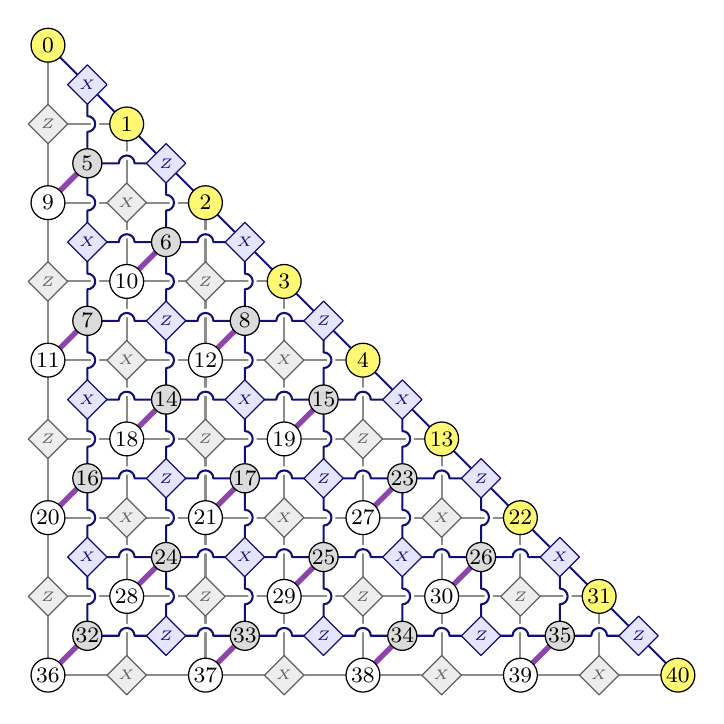
\begin{tikzpicture}[x=1cm,y=1cm,line cap=round,line join=round]
\draw[botline,line width=0.75pt] (0,-1) -- (0,-0);
\draw[botline,line width=0.75pt] (0,-1) -- (1,-1);
\draw[botline,line width=0.75pt] (0,-1) -- (0,-2);
\draw[botline,line width=0.75pt] (1,-2) -- (1,-1);
\draw[botline,line width=0.75pt] (1,-2) -- (2,-2);
\draw[botline,line width=0.75pt] (1,-2) -- (0,-2);
\draw[botline,line width=0.75pt] (1,-2) -- (1,-3);
\draw[botline,line width=0.75pt] (0,-3) -- (0,-2);
\draw[botline,line width=0.75pt] (0,-3) -- (1,-3);
\draw[botline,line width=0.75pt] (0,-3) -- (0,-4);
\draw[botline,line width=0.75pt] (2,-3) -- (2,-2);
\draw[botline,line width=0.75pt] (2,-3) -- (3,-3);
\draw[botline,line width=0.75pt] (2,-3) -- (1,-3);
\draw[botline,line width=0.75pt] (2,-3) -- (2,-4);
\draw[botline,line width=0.75pt] (1,-4) -- (1,-3);
\draw[botline,line width=0.75pt] (1,-4) -- (0,-4);
\draw[botline,line width=0.75pt] (1,-4) -- (2,-4);
\draw[botline,line width=0.75pt] (1,-4) -- (1,-5);
\draw[botline,line width=0.75pt] (3,-4) -- (3,-3);
\draw[botline,line width=0.75pt] (3,-4) -- (4,-4);
\draw[botline,line width=0.75pt] (3,-4) -- (2,-4);
\draw[botline,line width=0.75pt] (3,-4) -- (3,-5);
\draw[botline,line width=0.75pt] (0,-5) -- (0,-4);
\draw[botline,line width=0.75pt] (0,-5) -- (1,-5);
\draw[botline,line width=0.75pt] (0,-5) -- (0,-6);
\draw[botline,line width=0.75pt] (2,-5) -- (2,-4);
\draw[botline,line width=0.75pt] (2,-5) -- (1,-5);
\draw[botline,line width=0.75pt] (2,-5) -- (3,-5);
\draw[botline,line width=0.75pt] (2,-5) -- (2,-6);
\draw[botline,line width=0.75pt] (4,-5) -- (4,-4);
\draw[botline,line width=0.75pt] (4,-5) -- (5,-5);
\draw[botline,line width=0.75pt] (4,-5) -- (3,-5);
\draw[botline,line width=0.75pt] (4,-5) -- (4,-6);
\draw[botline,line width=0.75pt] (1,-6) -- (1,-5);
\draw[botline,line width=0.75pt] (1,-6) -- (0,-6);
\draw[botline,line width=0.75pt] (1,-6) -- (2,-6);
\draw[botline,line width=0.75pt] (1,-6) -- (1,-7);
\draw[botline,line width=0.75pt] (3,-6) -- (3,-5);
\draw[botline,line width=0.75pt] (3,-6) -- (2,-6);
\draw[botline,line width=0.75pt] (3,-6) -- (4,-6);
\draw[botline,line width=0.75pt] (3,-6) -- (3,-7);
\draw[botline,line width=0.75pt] (5,-6) -- (5,-5);
\draw[botline,line width=0.75pt] (5,-6) -- (6,-6);
\draw[botline,line width=0.75pt] (5,-6) -- (4,-6);
\draw[botline,line width=0.75pt] (5,-6) -- (5,-7);
\draw[botline,line width=0.75pt] (0,-7) -- (0,-6);
\draw[botline,line width=0.75pt] (0,-7) -- (1,-7);
\draw[botline,line width=0.75pt] (0,-7) -- (0,-8);
\draw[botline,line width=0.75pt] (2,-7) -- (2,-6);
\draw[botline,line width=0.75pt] (2,-7) -- (1,-7);
\draw[botline,line width=0.75pt] (2,-7) -- (3,-7);
\draw[botline,line width=0.75pt] (2,-7) -- (2,-8);
\draw[botline,line width=0.75pt] (4,-7) -- (4,-6);
\draw[botline,line width=0.75pt] (4,-7) -- (3,-7);
\draw[botline,line width=0.75pt] (4,-7) -- (5,-7);
\draw[botline,line width=0.75pt] (4,-7) -- (4,-8);
\draw[botline,line width=0.75pt] (6,-7) -- (6,-6);
\draw[botline,line width=0.75pt] (6,-7) -- (5,-7);
\draw[botline,line width=0.75pt] (6,-7) -- (7,-7);
\draw[botline,line width=0.75pt] (6,-7) -- (6,-8);
\draw[botline,line width=0.75pt] (1,-8) -- (1,-7);
\draw[botline,line width=0.75pt] (1,-8) -- (0,-8);
\draw[botline,line width=0.75pt] (1,-8) -- (2,-8);
\draw[botline,line width=0.75pt] (3,-8) -- (3,-7);
\draw[botline,line width=0.75pt] (3,-8) -- (2,-8);
\draw[botline,line width=0.75pt] (3,-8) -- (4,-8);
\draw[botline,line width=0.75pt] (5,-8) -- (5,-7);
\draw[botline,line width=0.75pt] (5,-8) -- (4,-8);
\draw[botline,line width=0.75pt] (5,-8) -- (6,-8);
\draw[botline,line width=0.75pt] (7,-8) -- (7,-7);
\draw[botline,line width=0.75pt] (7,-8) -- (6,-8);
\draw[botline,line width=0.75pt] (7,-8) -- (8,-8);
\draw[pairline,line width=1.95pt] (0,-2) -- (0.5,-1.5);
\draw[pairline,line width=1.95pt] (1,-3) -- (1.5,-2.5);
\draw[pairline,line width=1.95pt] (0,-4) -- (0.5,-3.5);
\draw[pairline,line width=1.95pt] (2,-4) -- (2.5,-3.5);
\draw[pairline,line width=1.95pt] (1,-5) -- (1.5,-4.5);
\draw[pairline,line width=1.95pt] (3,-5) -- (3.5,-4.5);
\draw[pairline,line width=1.95pt] (0,-6) -- (0.5,-5.5);
\draw[pairline,line width=1.95pt] (2,-6) -- (2.5,-5.5);
\draw[pairline,line width=1.95pt] (4,-6) -- (4.5,-5.5);
\draw[pairline,line width=1.95pt] (1,-7) -- (1.5,-6.5);
\draw[pairline,line width=1.95pt] (3,-7) -- (3.5,-6.5);
\draw[pairline,line width=1.95pt] (5,-7) -- (5.5,-6.5);
\draw[pairline,line width=1.95pt] (0,-8) -- (0.5,-7.5);
\draw[pairline,line width=1.95pt] (2,-8) -- (2.5,-7.5);
\draw[pairline,line width=1.95pt] (4,-8) -- (4.5,-7.5);
\draw[pairline,line width=1.95pt] (6,-8) -- (6.5,-7.5);
\draw[topline,line width=0.75pt] (0.5,-0.5) -- (0,-0);
\draw[topline,line width=0.75pt] (0.5,-0.5) -- (1,-1);
\draw[white,line width=2.95pt,line cap=butt] (0.5,-0.9) arc[start angle=90,end angle=-90,radius=0.1];
\draw[topline,line width=0.75pt] (0.5,-0.5) -- (0.5,-0.9) arc[start angle=90,end angle=-90,radius=0.1] -- (0.5,-1.5);
\draw[topline,line width=0.75pt] (1.5,-1.5) -- (1,-1);
\draw[topline,line width=0.75pt] (1.5,-1.5) -- (2,-2);
\draw[white,line width=2.95pt,line cap=butt] (0.9,-1.5) arc[start angle=180,end angle=0,radius=0.1];
\draw[topline,line width=0.75pt] (0.5,-1.5) -- (0.9,-1.5) arc[start angle=180,end angle=0,radius=0.1] -- (1.5,-1.5);
\draw[white,line width=2.95pt,line cap=butt] (1.5,-1.9) arc[start angle=90,end angle=-90,radius=0.1];
\draw[topline,line width=0.75pt] (1.5,-1.5) -- (1.5,-1.9) arc[start angle=90,end angle=-90,radius=0.1] -- (1.5,-2.5);
\draw[white,line width=2.95pt,line cap=butt] (0.5,-1.9) arc[start angle=90,end angle=-90,radius=0.1];
\draw[topline,line width=0.75pt] (0.5,-1.5) -- (0.5,-1.9) arc[start angle=90,end angle=-90,radius=0.1] -- (0.5,-2.5);
\draw[white,line width=2.95pt,line cap=butt] (0.9,-2.5) arc[start angle=180,end angle=0,radius=0.1];
\draw[topline,line width=0.75pt] (0.5,-2.5) -- (0.9,-2.5) arc[start angle=180,end angle=0,radius=0.1] -- (1.5,-2.5);
\draw[white,line width=2.95pt,line cap=butt] (0.5,-2.9) arc[start angle=90,end angle=-90,radius=0.1];
\draw[topline,line width=0.75pt] (0.5,-2.5) -- (0.5,-2.9) arc[start angle=90,end angle=-90,radius=0.1] -- (0.5,-3.5);
\draw[topline,line width=0.75pt] (2.5,-2.5) -- (2,-2);
\draw[topline,line width=0.75pt] (2.5,-2.5) -- (3,-3);
\draw[white,line width=2.95pt,line cap=butt] (1.9,-2.5) arc[start angle=180,end angle=0,radius=0.1];
\draw[topline,line width=0.75pt] (1.5,-2.5) -- (1.9,-2.5) arc[start angle=180,end angle=0,radius=0.1] -- (2.5,-2.5);
\draw[white,line width=2.95pt,line cap=butt] (2.5,-2.9) arc[start angle=90,end angle=-90,radius=0.1];
\draw[topline,line width=0.75pt] (2.5,-2.5) -- (2.5,-2.9) arc[start angle=90,end angle=-90,radius=0.1] -- (2.5,-3.5);
\draw[white,line width=2.95pt,line cap=butt] (1.5,-2.9) arc[start angle=90,end angle=-90,radius=0.1];
\draw[topline,line width=0.75pt] (1.5,-2.5) -- (1.5,-2.9) arc[start angle=90,end angle=-90,radius=0.1] -- (1.5,-3.5);
\draw[white,line width=2.95pt,line cap=butt] (0.9,-3.5) arc[start angle=180,end angle=0,radius=0.1];
\draw[topline,line width=0.75pt] (0.5,-3.5) -- (0.9,-3.5) arc[start angle=180,end angle=0,radius=0.1] -- (1.5,-3.5);
\draw[white,line width=2.95pt,line cap=butt] (1.9,-3.5) arc[start angle=180,end angle=0,radius=0.1];
\draw[topline,line width=0.75pt] (1.5,-3.5) -- (1.9,-3.5) arc[start angle=180,end angle=0,radius=0.1] -- (2.5,-3.5);
\draw[white,line width=2.95pt,line cap=butt] (1.5,-3.9) arc[start angle=90,end angle=-90,radius=0.1];
\draw[topline,line width=0.75pt] (1.5,-3.5) -- (1.5,-3.9) arc[start angle=90,end angle=-90,radius=0.1] -- (1.5,-4.5);
\draw[topline,line width=0.75pt] (3.5,-3.5) -- (3,-3);
\draw[topline,line width=0.75pt] (3.5,-3.5) -- (4,-4);
\draw[white,line width=2.95pt,line cap=butt] (2.9,-3.5) arc[start angle=180,end angle=0,radius=0.1];
\draw[topline,line width=0.75pt] (2.5,-3.5) -- (2.9,-3.5) arc[start angle=180,end angle=0,radius=0.1] -- (3.5,-3.5);
\draw[white,line width=2.95pt,line cap=butt] (3.5,-3.9) arc[start angle=90,end angle=-90,radius=0.1];
\draw[topline,line width=0.75pt] (3.5,-3.5) -- (3.5,-3.9) arc[start angle=90,end angle=-90,radius=0.1] -- (3.5,-4.5);
\draw[white,line width=2.95pt,line cap=butt] (0.5,-3.9) arc[start angle=90,end angle=-90,radius=0.1];
\draw[topline,line width=0.75pt] (0.5,-3.5) -- (0.5,-3.9) arc[start angle=90,end angle=-90,radius=0.1] -- (0.5,-4.5);
\draw[white,line width=2.95pt,line cap=butt] (0.9,-4.5) arc[start angle=180,end angle=0,radius=0.1];
\draw[topline,line width=0.75pt] (0.5,-4.5) -- (0.9,-4.5) arc[start angle=180,end angle=0,radius=0.1] -- (1.5,-4.5);
\draw[white,line width=2.95pt,line cap=butt] (0.5,-4.9) arc[start angle=90,end angle=-90,radius=0.1];
\draw[topline,line width=0.75pt] (0.5,-4.5) -- (0.5,-4.9) arc[start angle=90,end angle=-90,radius=0.1] -- (0.5,-5.5);
\draw[white,line width=2.95pt,line cap=butt] (2.5,-3.9) arc[start angle=90,end angle=-90,radius=0.1];
\draw[topline,line width=0.75pt] (2.5,-3.5) -- (2.5,-3.9) arc[start angle=90,end angle=-90,radius=0.1] -- (2.5,-4.5);
\draw[white,line width=2.95pt,line cap=butt] (1.9,-4.5) arc[start angle=180,end angle=0,radius=0.1];
\draw[topline,line width=0.75pt] (1.5,-4.5) -- (1.9,-4.5) arc[start angle=180,end angle=0,radius=0.1] -- (2.5,-4.5);
\draw[white,line width=2.95pt,line cap=butt] (2.9,-4.5) arc[start angle=180,end angle=0,radius=0.1];
\draw[topline,line width=0.75pt] (2.5,-4.5) -- (2.9,-4.5) arc[start angle=180,end angle=0,radius=0.1] -- (3.5,-4.5);
\draw[white,line width=2.95pt,line cap=butt] (2.5,-4.9) arc[start angle=90,end angle=-90,radius=0.1];
\draw[topline,line width=0.75pt] (2.5,-4.5) -- (2.5,-4.9) arc[start angle=90,end angle=-90,radius=0.1] -- (2.5,-5.5);
\draw[topline,line width=0.75pt] (4.5,-4.5) -- (4,-4);
\draw[topline,line width=0.75pt] (4.5,-4.5) -- (5,-5);
\draw[white,line width=2.95pt,line cap=butt] (3.9,-4.5) arc[start angle=180,end angle=0,radius=0.1];
\draw[topline,line width=0.75pt] (3.5,-4.5) -- (3.9,-4.5) arc[start angle=180,end angle=0,radius=0.1] -- (4.5,-4.5);
\draw[white,line width=2.95pt,line cap=butt] (4.5,-4.9) arc[start angle=90,end angle=-90,radius=0.1];
\draw[topline,line width=0.75pt] (4.5,-4.5) -- (4.5,-4.9) arc[start angle=90,end angle=-90,radius=0.1] -- (4.5,-5.5);
\draw[white,line width=2.95pt,line cap=butt] (1.5,-4.9) arc[start angle=90,end angle=-90,radius=0.1];
\draw[topline,line width=0.75pt] (1.5,-4.5) -- (1.5,-4.9) arc[start angle=90,end angle=-90,radius=0.1] -- (1.5,-5.5);
\draw[white,line width=2.95pt,line cap=butt] (0.9,-5.5) arc[start angle=180,end angle=0,radius=0.1];
\draw[topline,line width=0.75pt] (0.5,-5.5) -- (0.9,-5.5) arc[start angle=180,end angle=0,radius=0.1] -- (1.5,-5.5);
\draw[white,line width=2.95pt,line cap=butt] (1.9,-5.5) arc[start angle=180,end angle=0,radius=0.1];
\draw[topline,line width=0.75pt] (1.5,-5.5) -- (1.9,-5.5) arc[start angle=180,end angle=0,radius=0.1] -- (2.5,-5.5);
\draw[white,line width=2.95pt,line cap=butt] (1.5,-5.9) arc[start angle=90,end angle=-90,radius=0.1];
\draw[topline,line width=0.75pt] (1.5,-5.5) -- (1.5,-5.9) arc[start angle=90,end angle=-90,radius=0.1] -- (1.5,-6.5);
\draw[white,line width=2.95pt,line cap=butt] (3.5,-4.9) arc[start angle=90,end angle=-90,radius=0.1];
\draw[topline,line width=0.75pt] (3.5,-4.5) -- (3.5,-4.9) arc[start angle=90,end angle=-90,radius=0.1] -- (3.5,-5.5);
\draw[white,line width=2.95pt,line cap=butt] (2.9,-5.5) arc[start angle=180,end angle=0,radius=0.1];
\draw[topline,line width=0.75pt] (2.5,-5.5) -- (2.9,-5.5) arc[start angle=180,end angle=0,radius=0.1] -- (3.5,-5.5);
\draw[white,line width=2.95pt,line cap=butt] (3.9,-5.5) arc[start angle=180,end angle=0,radius=0.1];
\draw[topline,line width=0.75pt] (3.5,-5.5) -- (3.9,-5.5) arc[start angle=180,end angle=0,radius=0.1] -- (4.5,-5.5);
\draw[white,line width=2.95pt,line cap=butt] (3.5,-5.9) arc[start angle=90,end angle=-90,radius=0.1];
\draw[topline,line width=0.75pt] (3.5,-5.5) -- (3.5,-5.9) arc[start angle=90,end angle=-90,radius=0.1] -- (3.5,-6.5);
\draw[topline,line width=0.75pt] (5.5,-5.5) -- (5,-5);
\draw[topline,line width=0.75pt] (5.5,-5.5) -- (6,-6);
\draw[white,line width=2.95pt,line cap=butt] (4.9,-5.5) arc[start angle=180,end angle=0,radius=0.1];
\draw[topline,line width=0.75pt] (4.5,-5.5) -- (4.9,-5.5) arc[start angle=180,end angle=0,radius=0.1] -- (5.5,-5.5);
\draw[white,line width=2.95pt,line cap=butt] (5.5,-5.9) arc[start angle=90,end angle=-90,radius=0.1];
\draw[topline,line width=0.75pt] (5.5,-5.5) -- (5.5,-5.9) arc[start angle=90,end angle=-90,radius=0.1] -- (5.5,-6.5);
\draw[white,line width=2.95pt,line cap=butt] (0.5,-5.9) arc[start angle=90,end angle=-90,radius=0.1];
\draw[topline,line width=0.75pt] (0.5,-5.5) -- (0.5,-5.9) arc[start angle=90,end angle=-90,radius=0.1] -- (0.5,-6.5);
\draw[white,line width=2.95pt,line cap=butt] (0.9,-6.5) arc[start angle=180,end angle=0,radius=0.1];
\draw[topline,line width=0.75pt] (0.5,-6.5) -- (0.9,-6.5) arc[start angle=180,end angle=0,radius=0.1] -- (1.5,-6.5);
\draw[white,line width=2.95pt,line cap=butt] (0.5,-6.9) arc[start angle=90,end angle=-90,radius=0.1];
\draw[topline,line width=0.75pt] (0.5,-6.5) -- (0.5,-6.9) arc[start angle=90,end angle=-90,radius=0.1] -- (0.5,-7.5);
\draw[white,line width=2.95pt,line cap=butt] (2.5,-5.9) arc[start angle=90,end angle=-90,radius=0.1];
\draw[topline,line width=0.75pt] (2.5,-5.5) -- (2.5,-5.9) arc[start angle=90,end angle=-90,radius=0.1] -- (2.5,-6.5);
\draw[white,line width=2.95pt,line cap=butt] (1.9,-6.5) arc[start angle=180,end angle=0,radius=0.1];
\draw[topline,line width=0.75pt] (1.5,-6.5) -- (1.9,-6.5) arc[start angle=180,end angle=0,radius=0.1] -- (2.5,-6.5);
\draw[white,line width=2.95pt,line cap=butt] (2.9,-6.5) arc[start angle=180,end angle=0,radius=0.1];
\draw[topline,line width=0.75pt] (2.5,-6.5) -- (2.9,-6.5) arc[start angle=180,end angle=0,radius=0.1] -- (3.5,-6.5);
\draw[white,line width=2.95pt,line cap=butt] (2.5,-6.9) arc[start angle=90,end angle=-90,radius=0.1];
\draw[topline,line width=0.75pt] (2.5,-6.5) -- (2.5,-6.9) arc[start angle=90,end angle=-90,radius=0.1] -- (2.5,-7.5);
\draw[white,line width=2.95pt,line cap=butt] (4.5,-5.9) arc[start angle=90,end angle=-90,radius=0.1];
\draw[topline,line width=0.75pt] (4.5,-5.5) -- (4.5,-5.9) arc[start angle=90,end angle=-90,radius=0.1] -- (4.5,-6.5);
\draw[white,line width=2.95pt,line cap=butt] (3.9,-6.5) arc[start angle=180,end angle=0,radius=0.1];
\draw[topline,line width=0.75pt] (3.5,-6.5) -- (3.9,-6.5) arc[start angle=180,end angle=0,radius=0.1] -- (4.5,-6.5);
\draw[white,line width=2.95pt,line cap=butt] (4.9,-6.5) arc[start angle=180,end angle=0,radius=0.1];
\draw[topline,line width=0.75pt] (4.5,-6.5) -- (4.9,-6.5) arc[start angle=180,end angle=0,radius=0.1] -- (5.5,-6.5);
\draw[white,line width=2.95pt,line cap=butt] (4.5,-6.9) arc[start angle=90,end angle=-90,radius=0.1];
\draw[topline,line width=0.75pt] (4.5,-6.5) -- (4.5,-6.9) arc[start angle=90,end angle=-90,radius=0.1] -- (4.5,-7.5);
\draw[topline,line width=0.75pt] (6.5,-6.5) -- (6,-6);
\draw[white,line width=2.95pt,line cap=butt] (5.9,-6.5) arc[start angle=180,end angle=0,radius=0.1];
\draw[topline,line width=0.75pt] (5.5,-6.5) -- (5.9,-6.5) arc[start angle=180,end angle=0,radius=0.1] -- (6.5,-6.5);
\draw[topline,line width=0.75pt] (6.5,-6.5) -- (7,-7);
\draw[white,line width=2.95pt,line cap=butt] (6.5,-6.9) arc[start angle=90,end angle=-90,radius=0.1];
\draw[topline,line width=0.75pt] (6.5,-6.5) -- (6.5,-6.9) arc[start angle=90,end angle=-90,radius=0.1] -- (6.5,-7.5);
\draw[white,line width=2.95pt,line cap=butt] (1.5,-6.9) arc[start angle=90,end angle=-90,radius=0.1];
\draw[topline,line width=0.75pt] (1.5,-6.5) -- (1.5,-6.9) arc[start angle=90,end angle=-90,radius=0.1] -- (1.5,-7.5);
\draw[white,line width=2.95pt,line cap=butt] (0.9,-7.5) arc[start angle=180,end angle=0,radius=0.1];
\draw[topline,line width=0.75pt] (0.5,-7.5) -- (0.9,-7.5) arc[start angle=180,end angle=0,radius=0.1] -- (1.5,-7.5);
\draw[white,line width=2.95pt,line cap=butt] (1.9,-7.5) arc[start angle=180,end angle=0,radius=0.1];
\draw[topline,line width=0.75pt] (1.5,-7.5) -- (1.9,-7.5) arc[start angle=180,end angle=0,radius=0.1] -- (2.5,-7.5);
\draw[white,line width=2.95pt,line cap=butt] (3.5,-6.9) arc[start angle=90,end angle=-90,radius=0.1];
\draw[topline,line width=0.75pt] (3.5,-6.5) -- (3.5,-6.9) arc[start angle=90,end angle=-90,radius=0.1] -- (3.5,-7.5);
\draw[white,line width=2.95pt,line cap=butt] (2.9,-7.5) arc[start angle=180,end angle=0,radius=0.1];
\draw[topline,line width=0.75pt] (2.5,-7.5) -- (2.9,-7.5) arc[start angle=180,end angle=0,radius=0.1] -- (3.5,-7.5);
\draw[white,line width=2.95pt,line cap=butt] (3.9,-7.5) arc[start angle=180,end angle=0,radius=0.1];
\draw[topline,line width=0.75pt] (3.5,-7.5) -- (3.9,-7.5) arc[start angle=180,end angle=0,radius=0.1] -- (4.5,-7.5);
\draw[white,line width=2.95pt,line cap=butt] (5.5,-6.9) arc[start angle=90,end angle=-90,radius=0.1];
\draw[topline,line width=0.75pt] (5.5,-6.5) -- (5.5,-6.9) arc[start angle=90,end angle=-90,radius=0.1] -- (5.5,-7.5);
\draw[white,line width=2.95pt,line cap=butt] (4.9,-7.5) arc[start angle=180,end angle=0,radius=0.1];
\draw[topline,line width=0.75pt] (4.5,-7.5) -- (4.9,-7.5) arc[start angle=180,end angle=0,radius=0.1] -- (5.5,-7.5);
\draw[white,line width=2.95pt,line cap=butt] (5.9,-7.5) arc[start angle=180,end angle=0,radius=0.1];
\draw[topline,line width=0.75pt] (5.5,-7.5) -- (5.9,-7.5) arc[start angle=180,end angle=0,radius=0.1] -- (6.5,-7.5);
\draw[topline,line width=0.75pt] (7.5,-7.5) -- (7,-7);
\draw[white,line width=2.95pt,line cap=butt] (6.9,-7.5) arc[start angle=180,end angle=0,radius=0.1];
\draw[topline,line width=0.75pt] (6.5,-7.5) -- (6.9,-7.5) arc[start angle=180,end angle=0,radius=0.1] -- (7.5,-7.5);
\draw[topline,line width=0.75pt] (7.5,-7.5) -- (8,-8);
\draw[botanc,line width=0.45pt] (-0.25,-1) -- (0,-0.75) -- (0.25,-1) -- (0,-1.25) -- cycle;
\node[anclabel,botanctext] at (0,-1) {\tiny $Z$};
\draw[botanc,line width=0.45pt] (0.75,-2) -- (1,-1.75) -- (1.25,-2) -- (1,-2.25) -- cycle;
\node[anclabel,botanctext] at (1,-2) {\tiny $X$};
\draw[botanc,line width=0.45pt] (-0.25,-3) -- (0,-2.75) -- (0.25,-3) -- (0,-3.25) -- cycle;
\node[anclabel,botanctext] at (0,-3) {\tiny $Z$};
\draw[botanc,line width=0.45pt] (1.75,-3) -- (2,-2.75) -- (2.25,-3) -- (2,-3.25) -- cycle;
\node[anclabel,botanctext] at (2,-3) {\tiny $Z$};
\draw[botanc,line width=0.45pt] (0.75,-4) -- (1,-3.75) -- (1.25,-4) -- (1,-4.25) -- cycle;
\node[anclabel,botanctext] at (1,-4) {\tiny $X$};
\draw[botanc,line width=0.45pt] (2.75,-4) -- (3,-3.75) -- (3.25,-4) -- (3,-4.25) -- cycle;
\node[anclabel,botanctext] at (3,-4) {\tiny $X$};
\draw[botanc,line width=0.45pt] (-0.25,-5) -- (0,-4.75) -- (0.25,-5) -- (0,-5.25) -- cycle;
\node[anclabel,botanctext] at (0,-5) {\tiny $Z$};
\draw[botanc,line width=0.45pt] (1.75,-5) -- (2,-4.75) -- (2.25,-5) -- (2,-5.25) -- cycle;
\node[anclabel,botanctext] at (2,-5) {\tiny $Z$};
\draw[botanc,line width=0.45pt] (3.75,-5) -- (4,-4.75) -- (4.25,-5) -- (4,-5.25) -- cycle;
\node[anclabel,botanctext] at (4,-5) {\tiny $Z$};
\draw[botanc,line width=0.45pt] (0.75,-6) -- (1,-5.75) -- (1.25,-6) -- (1,-6.25) -- cycle;
\node[anclabel,botanctext] at (1,-6) {\tiny $X$};
\draw[botanc,line width=0.45pt] (2.75,-6) -- (3,-5.75) -- (3.25,-6) -- (3,-6.25) -- cycle;
\node[anclabel,botanctext] at (3,-6) {\tiny $X$};
\draw[botanc,line width=0.45pt] (4.75,-6) -- (5,-5.75) -- (5.25,-6) -- (5,-6.25) -- cycle;
\node[anclabel,botanctext] at (5,-6) {\tiny $X$};
\draw[botanc,line width=0.45pt] (-0.25,-7) -- (0,-6.75) -- (0.25,-7) -- (0,-7.25) -- cycle;
\node[anclabel,botanctext] at (0,-7) {\tiny $Z$};
\draw[botanc,line width=0.45pt] (1.75,-7) -- (2,-6.75) -- (2.25,-7) -- (2,-7.25) -- cycle;
\node[anclabel,botanctext] at (2,-7) {\tiny $Z$};
\draw[botanc,line width=0.45pt] (3.75,-7) -- (4,-6.75) -- (4.25,-7) -- (4,-7.25) -- cycle;
\node[anclabel,botanctext] at (4,-7) {\tiny $Z$};
\draw[botanc,line width=0.45pt] (5.75,-7) -- (6,-6.75) -- (6.25,-7) -- (6,-7.25) -- cycle;
\node[anclabel,botanctext] at (6,-7) {\tiny $Z$};
\draw[botanc,line width=0.45pt] (0.75,-8) -- (1,-7.75) -- (1.25,-8) -- (1,-8.25) -- cycle;
\node[anclabel,botanctext] at (1,-8) {\tiny $X$};
\draw[botanc,line width=0.45pt] (2.75,-8) -- (3,-7.75) -- (3.25,-8) -- (3,-8.25) -- cycle;
\node[anclabel,botanctext] at (3,-8) {\tiny $X$};
\draw[botanc,line width=0.45pt] (4.75,-8) -- (5,-7.75) -- (5.25,-8) -- (5,-8.25) -- cycle;
\node[anclabel,botanctext] at (5,-8) {\tiny $X$};
\draw[botanc,line width=0.45pt] (6.75,-8) -- (7,-7.75) -- (7.25,-8) -- (7,-8.25) -- cycle;
\node[anclabel,botanctext] at (7,-8) {\tiny $X$};
\draw[topanc,line width=0.45pt] (0.25,-0.5) -- (0.5,-0.25) -- (0.75,-0.5) -- (0.5,-0.75) -- cycle;
\node[anclabel,topanctext] at (0.5,-0.5) {\tiny $X$};
\draw[topanc,line width=0.45pt] (1.25,-1.5) -- (1.5,-1.25) -- (1.75,-1.5) -- (1.5,-1.75) -- cycle;
\node[anclabel,topanctext] at (1.5,-1.5) {\tiny $Z$};
\draw[topanc,line width=0.45pt] (0.25,-2.5) -- (0.5,-2.25) -- (0.75,-2.5) -- (0.5,-2.75) -- cycle;
\node[anclabel,topanctext] at (0.5,-2.5) {\tiny $X$};
\draw[topanc,line width=0.45pt] (2.25,-2.5) -- (2.5,-2.25) -- (2.75,-2.5) -- (2.5,-2.75) -- cycle;
\node[anclabel,topanctext] at (2.5,-2.5) {\tiny $X$};
\draw[topanc,line width=0.45pt] (1.25,-3.5) -- (1.5,-3.25) -- (1.75,-3.5) -- (1.5,-3.75) -- cycle;
\node[anclabel,topanctext] at (1.5,-3.5) {\tiny $Z$};
\draw[topanc,line width=0.45pt] (3.25,-3.5) -- (3.5,-3.25) -- (3.75,-3.5) -- (3.5,-3.75) -- cycle;
\node[anclabel,topanctext] at (3.5,-3.5) {\tiny $Z$};
\draw[topanc,line width=0.45pt] (0.25,-4.5) -- (0.5,-4.25) -- (0.75,-4.5) -- (0.5,-4.75) -- cycle;
\node[anclabel,topanctext] at (0.5,-4.5) {\tiny $X$};
\draw[topanc,line width=0.45pt] (2.25,-4.5) -- (2.5,-4.25) -- (2.75,-4.5) -- (2.5,-4.75) -- cycle;
\node[anclabel,topanctext] at (2.5,-4.5) {\tiny $X$};
\draw[topanc,line width=0.45pt] (4.25,-4.5) -- (4.5,-4.25) -- (4.75,-4.5) -- (4.5,-4.75) -- cycle;
\node[anclabel,topanctext] at (4.5,-4.5) {\tiny $X$};
\draw[topanc,line width=0.45pt] (1.25,-5.5) -- (1.5,-5.25) -- (1.75,-5.5) -- (1.5,-5.75) -- cycle;
\node[anclabel,topanctext] at (1.5,-5.5) {\tiny $Z$};
\draw[topanc,line width=0.45pt] (3.25,-5.5) -- (3.5,-5.25) -- (3.75,-5.5) -- (3.5,-5.75) -- cycle;
\node[anclabel,topanctext] at (3.5,-5.5) {\tiny $Z$};
\draw[topanc,line width=0.45pt] (5.25,-5.5) -- (5.5,-5.25) -- (5.75,-5.5) -- (5.5,-5.75) -- cycle;
\node[anclabel,topanctext] at (5.5,-5.5) {\tiny $Z$};
\draw[topanc,line width=0.45pt] (0.25,-6.5) -- (0.5,-6.25) -- (0.75,-6.5) -- (0.5,-6.75) -- cycle;
\node[anclabel,topanctext] at (0.5,-6.5) {\tiny $X$};
\draw[topanc,line width=0.45pt] (2.25,-6.5) -- (2.5,-6.25) -- (2.75,-6.5) -- (2.5,-6.75) -- cycle;
\node[anclabel,topanctext] at (2.5,-6.5) {\tiny $X$};
\draw[topanc,line width=0.45pt] (4.25,-6.5) -- (4.5,-6.25) -- (4.75,-6.5) -- (4.5,-6.75) -- cycle;
\node[anclabel,topanctext] at (4.5,-6.5) {\tiny $X$};
\draw[topanc,line width=0.45pt] (6.25,-6.5) -- (6.5,-6.25) -- (6.75,-6.5) -- (6.5,-6.75) -- cycle;
\node[anclabel,topanctext] at (6.5,-6.5) {\tiny $X$};
\draw[topanc,line width=0.45pt] (1.25,-7.5) -- (1.5,-7.25) -- (1.75,-7.5) -- (1.5,-7.75) -- cycle;
\node[anclabel,topanctext] at (1.5,-7.5) {\tiny $Z$};
\draw[topanc,line width=0.45pt] (3.25,-7.5) -- (3.5,-7.25) -- (3.75,-7.5) -- (3.5,-7.75) -- cycle;
\node[anclabel,topanctext] at (3.5,-7.5) {\tiny $Z$};
\draw[topanc,line width=0.45pt] (5.25,-7.5) -- (5.5,-7.25) -- (5.75,-7.5) -- (5.5,-7.75) -- cycle;
\node[anclabel,topanctext] at (5.5,-7.5) {\tiny $Z$};
\draw[topanc,line width=0.45pt] (7.25,-7.5) -- (7.5,-7.25) -- (7.75,-7.5) -- (7.5,-7.75) -- cycle;
\node[anclabel,topanctext] at (7.5,-7.5) {\tiny $Z$};
\draw[foldq,line width=0.45pt] (0,-0) circle[radius=0.215];
\node[qlabel] at (0,-0) {\footnotesize 0};
\draw[foldq,line width=0.45pt] (1,-1) circle[radius=0.215];
\node[qlabel] at (1,-1) {\footnotesize 1};
\draw[foldq,line width=0.45pt] (2,-2) circle[radius=0.215];
\node[qlabel] at (2,-2) {\footnotesize 2};
\draw[foldq,line width=0.45pt] (3,-3) circle[radius=0.215];
\node[qlabel] at (3,-3) {\footnotesize 3};
\draw[foldq,line width=0.45pt] (4,-4) circle[radius=0.215];
\node[qlabel] at (4,-4) {\footnotesize 4};
\draw[topq,line width=0.45pt] (0.5,-1.5) circle[radius=0.1849];
\node[qlabel] at (0.5,-1.5) {\footnotesize 5};
\draw[topq,line width=0.45pt] (1.5,-2.5) circle[radius=0.1849];
\node[qlabel] at (1.5,-2.5) {\footnotesize 6};
\draw[topq,line width=0.45pt] (0.5,-3.5) circle[radius=0.1849];
\node[qlabel] at (0.5,-3.5) {\footnotesize 7};
\draw[topq,line width=0.45pt] (2.5,-3.5) circle[radius=0.1849];
\node[qlabel] at (2.5,-3.5) {\footnotesize 8};
\draw[botq,line width=0.45pt] (0,-2) circle[radius=0.215];
\node[qlabel] at (0,-2) {\footnotesize 9};
\draw[botq,line width=0.45pt] (1,-3) circle[radius=0.215];
\node[qlabel] at (1,-3) {\footnotesize 10};
\draw[botq,line width=0.45pt] (0,-4) circle[radius=0.215];
\node[qlabel] at (0,-4) {\footnotesize 11};
\draw[botq,line width=0.45pt] (2,-4) circle[radius=0.215];
\node[qlabel] at (2,-4) {\footnotesize 12};
\draw[foldq,line width=0.45pt] (5,-5) circle[radius=0.215];
\node[qlabel] at (5,-5) {\footnotesize 13};
\draw[topq,line width=0.45pt] (1.5,-4.5) circle[radius=0.1849];
\node[qlabel] at (1.5,-4.5) {\footnotesize 14};
\draw[topq,line width=0.45pt] (3.5,-4.5) circle[radius=0.1849];
\node[qlabel] at (3.5,-4.5) {\footnotesize 15};
\draw[topq,line width=0.45pt] (0.5,-5.5) circle[radius=0.1849];
\node[qlabel] at (0.5,-5.5) {\footnotesize 16};
\draw[topq,line width=0.45pt] (2.5,-5.5) circle[radius=0.1849];
\node[qlabel] at (2.5,-5.5) {\footnotesize 17};
\draw[botq,line width=0.45pt] (1,-5) circle[radius=0.215];
\node[qlabel] at (1,-5) {\footnotesize 18};
\draw[botq,line width=0.45pt] (3,-5) circle[radius=0.215];
\node[qlabel] at (3,-5) {\footnotesize 19};
\draw[botq,line width=0.45pt] (0,-6) circle[radius=0.215];
\node[qlabel] at (0,-6) {\footnotesize 20};
\draw[botq,line width=0.45pt] (2,-6) circle[radius=0.215];
\node[qlabel] at (2,-6) {\footnotesize 21};
\draw[foldq,line width=0.45pt] (6,-6) circle[radius=0.215];
\node[qlabel] at (6,-6) {\footnotesize 22};
\draw[topq,line width=0.45pt] (4.5,-5.5) circle[radius=0.1849];
\node[qlabel] at (4.5,-5.5) {\footnotesize 23};
\draw[topq,line width=0.45pt] (1.5,-6.5) circle[radius=0.1849];
\node[qlabel] at (1.5,-6.5) {\footnotesize 24};
\draw[topq,line width=0.45pt] (3.5,-6.5) circle[radius=0.1849];
\node[qlabel] at (3.5,-6.5) {\footnotesize 25};
\draw[topq,line width=0.45pt] (5.5,-6.5) circle[radius=0.1849];
\node[qlabel] at (5.5,-6.5) {\footnotesize 26};
\draw[botq,line width=0.45pt] (4,-6) circle[radius=0.215];
\node[qlabel] at (4,-6) {\footnotesize 27};
\draw[botq,line width=0.45pt] (1,-7) circle[radius=0.215];
\node[qlabel] at (1,-7) {\footnotesize 28};
\draw[botq,line width=0.45pt] (3,-7) circle[radius=0.215];
\node[qlabel] at (3,-7) {\footnotesize 29};
\draw[botq,line width=0.45pt] (5,-7) circle[radius=0.215];
\node[qlabel] at (5,-7) {\footnotesize 30};
\draw[foldq,line width=0.45pt] (7,-7) circle[radius=0.215];
\node[qlabel] at (7,-7) {\footnotesize 31};
\draw[topq,line width=0.45pt] (0.5,-7.5) circle[radius=0.1849];
\node[qlabel] at (0.5,-7.5) {\footnotesize 32};
\draw[topq,line width=0.45pt] (2.5,-7.5) circle[radius=0.1849];
\node[qlabel] at (2.5,-7.5) {\footnotesize 33};
\draw[topq,line width=0.45pt] (4.5,-7.5) circle[radius=0.1849];
\node[qlabel] at (4.5,-7.5) {\footnotesize 34};
\draw[topq,line width=0.45pt] (6.5,-7.5) circle[radius=0.1849];
\node[qlabel] at (6.5,-7.5) {\footnotesize 35};
\draw[botq,line width=0.45pt] (0,-8) circle[radius=0.215];
\node[qlabel] at (0,-8) {\footnotesize 36};
\draw[botq,line width=0.45pt] (2,-8) circle[radius=0.215];
\node[qlabel] at (2,-8) {\footnotesize 37};
\draw[botq,line width=0.45pt] (4,-8) circle[radius=0.215];
\node[qlabel] at (4,-8) {\footnotesize 38};
\draw[botq,line width=0.45pt] (6,-8) circle[radius=0.215];
\node[qlabel] at (6,-8) {\footnotesize 39};
\draw[foldq,line width=0.45pt] (8,-8) circle[radius=0.215];
\node[qlabel] at (8,-8) {\footnotesize 40};
\end{tikzpicture}
\\[2pt] {\small $d=5$}\end{minipage}
\caption{The layout for $d=2$ to $5$ at one scale, drawn as in Fig.~\ref{fig:d3}(b). Each
distance contains the previous one as its upper-left corner, up to the numbering.}
\label{fig:family}
\end{figure}

\section{What the chip has to provide}
\label{sec:chip}

\begin{itemize}
\item \textbf{Two coupler lengths.} Couplers between an ancilla and a data qubit have length
$a$, except the $4(d-1)$ at the fold, which have length $a/\sqrt2$ like the pair couplers.
\item \textbf{Five couplers on a data qubit.} A data qubit away from the fold and from the edge
couples to four ancillas and to its partner. Fold qubits and ancillas have at most four
couplers. Square-lattice processors give each qubit four, so the fifth port is the one new
element.
\item \textbf{One kind of crossover.} Two couplers cross at right angles at their midpoints, and
no coupler is crossed twice. An air bridge on a single chip~\cite{Chen2014} and a flip-chip
stack with one layer per chip~\cite{Rosenberg2017,Foxen2018} are the two standard ways to build
it. In the flip-chip version the pair couplers and the couplers of the top-layer ancillas at
the fold cross the gap between the chips.
\item \textbf{Spacing.} A top-layer site sits $a/\sqrt2$ from the corners of its cell, four in
the bulk and three on the fold. A top-layer data qubit couples to one of them, a top-layer
ancilla at the fold to two, and a top-layer ancilla in the bulk to none. Stray coupling to the other corners sets how small $a$
can be.
\item \textbf{Three frequency groups.} A pair coupler closes a loop with an odd number of
couplers, five for a pair next to the fold, so two groups do not suffice. Three do: the ancillas,
the fold qubits with the bottom-layer data qubits, and the top-layer data qubits. No coupler
joins two qubits of one group.
\item \textbf{The SWAPs can be free.} Exchanging the two layers, with the fold qubits fixed,
maps the coupling graph onto itself. The SWAPs of logical $H$ can therefore be a relabelling of
the layers, after which every ancilla measures the other type of check. The pair couplers then
serve the CZ gates of logical $S$ only.
\end{itemize}

The note leaves out the control and readout lines. Every qubit needs them, and in a triangle
this dense they have to reach the interior from above or below the plane of the chip. It also gives no gate
schedule. The four-step schedule of the unrotated code applies unchanged, because the layout
moves qubits and does not change which ancilla touches which data qubit.

\section{Memory under circuit-level noise}
\label{sec:memory}

Folding moves qubits but keeps every coupling between an ancilla and its data qubits, so a check
round on this layout is a check round of the unrotated surface code. We simulated memory
experiments of $d$ rounds, in the $X$ and $Z$ bases, under the SD6 and SI1000 models of
Ref.~\cite{Gidney2021}, and decoded them by minimum-weight perfect matching (stim, sinter and
pymatching). The rotated surface code, built by the same code with the same noise, schedule rules
and decoder, is the baseline. Every check visits its neighbours north, west, east, south; the rotated
code uses the usual N- and Z-shaped orders. For both codes and both bases we checked that every
detector is deterministic and that the shortest logical error of the circuit has weight $d$, and for
the folded code that every two-qubit gate acts on a coupler of this layout.
Table~\ref{tab:memory} and Fig.~\ref{fig:memory} summarise the results; the details are in
\texttt{memory/README.md}.

\begin{table}[!ht]
\centering
\begin{tabular}{@{}llcc@{}}
\toprule
 & & folded & rotated\\
\midrule
threshold per round ($d=9$ and $11$ cross) & SD6 & 0.70\% & 0.73\%\\
 & SI1000 & 0.51\% & 0.54\%\\
$\Lambda$ at $p=0.1\%$ ($d=5$ to $11$) & SD6 & 11.3 & 6.7\\
 & SI1000 & 9.3 & 5.7\\
qubits for a teraquop memory at $p=0.1\%$ & SD6 & 2025 ($d=23$) & 1681 ($d=29$)\\
 & SI1000 & 2401 ($d=25$) & 2177 ($d=33$)\\
\bottomrule
\end{tabular}
\caption{Memory of the folded and the rotated surface code. $\Lambda$ is the suppression of the
logical error per round when $d$ grows by two. A teraquop memory fails with probability
$10^{-12}$ per block of $d$ rounds~\cite{Gidney2021}; its size comes from the fitted $\Lambda$.}
\label{tab:memory}
\end{table}

Three results follow. First, the thresholds agree within the step of our grid of $p$. Second, at
equal distance the folded code fails less often, because the unrotated lattice has fewer logical
strings of minimum weight. Third, at equal qubit count the rotated code wins, since it reaches
distance $d$ with $2d^2-1$ qubits against $(2d-1)^2$. For a teraquop memory at $p=0.1\%$ the
folded code needs 20\% more qubits under SD6 and 10\% more under SI1000.

The folded code buys these qubits back with its logical gates (Fig.~\ref{fig:memory}, right). A
fold-transversal $H$ between every two rounds is a Hadamard layer on the data qubits, done in the
time step where the ancillas change basis, followed by a swap of the check roles; it leaves the
error per round unchanged (ratio $1.00\pm0.05$ under SD6). A fold-transversal $S$ between every two
rounds adds one layer of CZ gates on the $(d-1)^2$ fold pairs and raises the error per round by a
factor 1.2 to 1.7 for $d=3$ to $9$ and $p=0.1$ to $0.3\%$, about half a round of memory per gate.
On the rotated code neither gate is transversal on fixed hardware: $H$ needs a patch rotation, and
Moussa estimates a logical $S$ at about $72d^3$ qubit-rounds~\cite{Moussa2016}.

We ran the $S$ memories in the $Z$ basis only. There a CZ never turns a $Z$ error into an $X$ error,
so matching the $Z$ checks alone decodes $Z_L$. In the $X$ basis an $X$ error between two gates
becomes a $Z$ error on its mirror qubit and flips $X_L$, and only the $Z$ checks see it; decoding
it needs both sectors at once (correlated decoding of transversal gates), which we leave for later.

\begin{figure}[!ht]
\centering
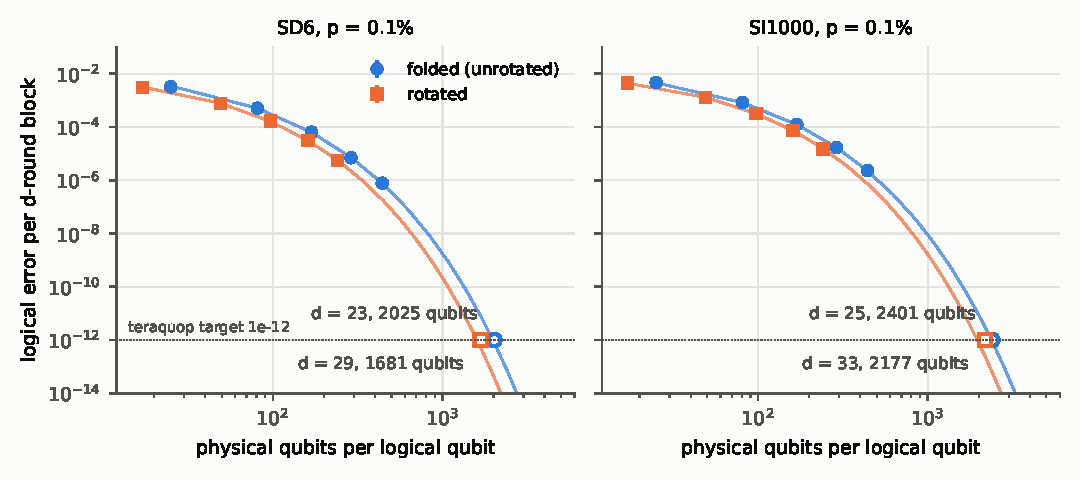
\includegraphics[width=\textwidth]{memory/figures/memory-footprint.pdf}\\[4pt]
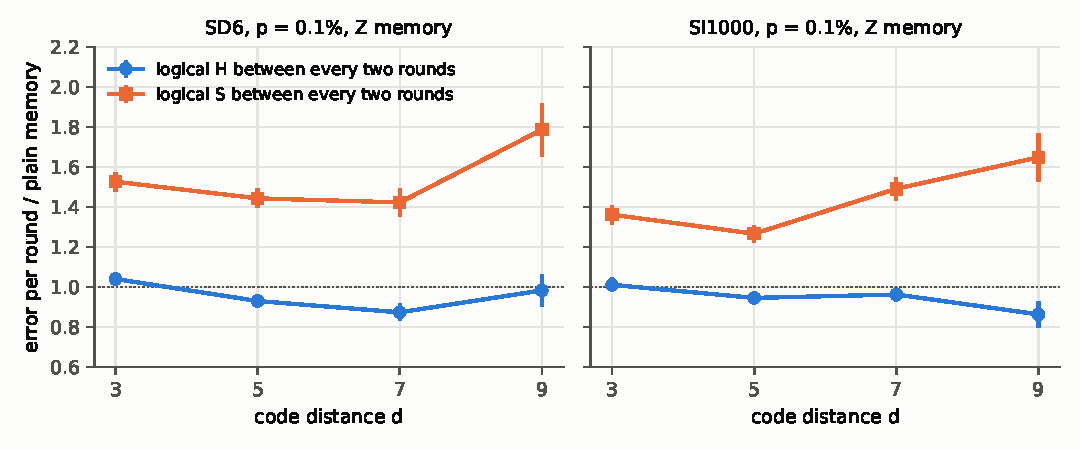
\includegraphics[width=\textwidth]{memory/figures/memory-gates.pdf}
\caption{Top: logical error per block of $d$ rounds against the number of physical qubits at
$p=0.1\%$; points are simulations ($d=3$ to $11$), lines the $\Lambda$ fits, open symbols the
teraquop sizes. Bottom: error per round of the folded code with a fold-transversal $H$ or $S$
between every two rounds, divided by the plain memory, at $p=0.1\%$ in the $Z$ basis.}
\label{fig:memory}
\end{figure}

\section{Numbering, checks and files}

\paragraph{Numbering.} The data qubits are numbered in blocks that are alternately $d$ and
$d-1$ long, like the rows of the unrotated code. Number the first $d$ fold qubits $0$ to $d-1$,
starting at the corner $(0,0)$. Take the bottom-layer data qubits in reading order, top row first and left to right,
and cut the list into $d-1$ groups of $d-1$. For each group in turn, number the top-layer
partners of the group, then the group itself, then the next fold qubit. At $d=2$ this gives the
labels of the LRB paper: fold qubits 0, 1, 4, the pair 2--3, and checks on $\{0,1,3\}$,
$\{1,2,4\}$ ($Z$ type) and $\{0,1,2\}$, $\{1,3,4\}$ ($X$ type). At $d=3$ it gives the labels of
the hand-drawn sketch this note started from. For larger $d$ the rule is only a convention.
The data files give the coordinates of every qubit, so another numbering is a relabelling.
Table~\ref{tab:checks} lists the check of every ancilla for $d=2$ and $d=3$.

\paragraph{Checks.} For $d=2$ to $6$ the script verifies the counts of Table~\ref{tab:counts};
that the $X$ and $Z$ checks commute and encode one logical qudit, for qubits and qutrits; that
the fold maps the $X$ checks onto the $Z$ checks; that logical $H$ and $S$ as given above
preserve the stabilizer group and act correctly on the logical operators, up to Pauli
corrections, for qubits and qutrits; the two coupler lengths; the position and number of the
crossovers; that the coupling graph is planar only at $d=2$; that each distance contains the
previous one; the three frequency groups; and the layer-exchange symmetry. For $d\le5$ it also confirms by exhaustive search that no logical operator of the
qubit code has weight below $d$.

\paragraph{Files.} Everything is in \texttt{layouts/folded-surface-code/} of the repository.
\begin{itemize}
\item \texttt{gen\_layout.py} builds and checks the layout for any $d$ and writes the data files
and the TikZ sources. \texttt{python gen\_layout.py 8} extends the data files to $d=8$.
\item \texttt{data/layout-d2.json} to \texttt{layout-d6.json} list every qubit with its
coordinates, role and partner, every ancilla with its check type and data qubits, every coupler
and every crossover. For qudits they also give one valid choice of exponents for the checks. At
$d=2$, after inverting both Paulis on $q_1$, this choice gives $G_1$, $G_2$ and the inverses of
$G_3$, $G_4$ of the LRB paper, which generate the same stabilizer group.
\item \texttt{layout-d2.pdf} to \texttt{layout-d6.pdf} are the pictures alone, one per distance.
\item \texttt{figures/} holds the TikZ sources, and \texttt{layout-style.tex} their styles.
\item \texttt{memory/} holds the memory study: circuits, checks, runs, results and figures.
\end{itemize}

\begin{table}[!ht]
\centering
\small
\begin{tabular}[t]{@{}llll@{}}
\multicolumn{4}{@{}l}{$d=2$}\\
\toprule
layer & check & position $(x,y)/a$ & data qubits\\
\midrule
\rawinput{figures/checks-d2.tex}
\bottomrule
\end{tabular}
\hspace{1.2cm}
\begin{tabular}[t]{@{}llll@{}}
\multicolumn{4}{@{}l}{$d=3$}\\
\toprule
layer & check & position $(x,y)/a$ & data qubits\\
\midrule
\rawinput{figures/checks-d3.tex}
\bottomrule
\end{tabular}
\caption{The check measured by each ancilla for $d=2$ and $d=3$, with positions as in
Fig.~\ref{fig:family}: $x$ to the right, $y$ downwards, origin at qubit~0.}
\label{tab:checks}
\end{table}

\begin{thebibliography}{9}
\bibitem{Gidney2021} C.~Gidney, M.~Newman, A.~Fowler and M.~Broughton, A fault-tolerant honeycomb
memory, Quantum \textbf{5}, 605 (2021), arXiv:2108.10457.
\bibitem{Moussa2016} J.~E. Moussa, Transversal Clifford gates on folded surface codes,
Phys. Rev. A \textbf{94}, 042316 (2016), arXiv:1603.02286.
\bibitem{Breuckmann2024} N.~P. Breuckmann and S.~Burton, Fold-transversal Clifford gates for
quantum codes, Quantum \textbf{8}, 1372 (2024), arXiv:2202.06647.
\bibitem{Chen2014} Z.~Chen \emph{et al.}, Fabrication and characterization of aluminum airbridges
for superconducting microwave circuits, Appl. Phys. Lett. \textbf{104}, 052602 (2014).
\bibitem{Rosenberg2017} D.~Rosenberg \emph{et al.}, 3D integrated superconducting qubits,
npj Quantum Inf. \textbf{3}, 42 (2017).
\bibitem{Foxen2018} B.~Foxen \emph{et al.}, Qubit compatible superconducting interconnects,
Quantum Sci. Technol. \textbf{3}, 014005 (2018).
\end{thebibliography}

\end{document}
